\chapter{Study of the Wobbling Motion via a Boson Description}
\label{extra-chapter-new-boson}

This last part will be focused on the wobbling phenomenon but with a different approach than Chapters \ref{chapter-4-aw1-formalism} ($\mathbf{W_1}$) and \ref{chapter-5-novel} ($\mathbf{W_2}$), as this method does not share the same foundational concepts. All the theoretical calculations and results shown here correspond to a publication made by the team for the nucleus $^{135}$Pr in Ref. \cite{raduta2020new}. In the first section, a set of results for the description of the angular momentum via boson operators are briefly recalled from the $\mathbf{W_0}$ formalism. In the second section, the Hamiltonian and its framework will be developed using the transformation laws from the previous section. Two different expansions for the total angular momentum are obtained through these boson calculations. Furthermore, the Jacobi elliptic functions are introduced and used to construct the potential energy for a triaxial rotor. By studying the first-order derivative for the elliptic potential, the critical points can be acquired. The points of local and global minima are of interest here, because a second-order expansion around them leads to analytical expressions for the total energy and wobbling frequency of the triaxial system. The third section invokes a semi-classical analysis, giving equations for the total energy in terms of the angular momentum components. Depending on the axis with the largest MOI of the triaxial rotor, three situations can occur, where each of the $1$-, $2$-, and $3$-axis have the largest MOI. Phase diagrams that show the energy function in terms of a polar representation for the a.m. components are constructed. These provide useful information regarding the stability of the wobbling motion. The electromagnetic transitions and their expressions are treated in the fourth section, while a comparison of the data concerning energies and transition probabilities between the model and the experimental measurements for $^{135}$Pr is given in the fifth section. Concluding remarks on this research are provided at the end of the chapter.

\section{Angular Momentum - Boson Representation}
\label{section-intro-boson-representation}

Besides the odd-mass case study performed by the team in Ref. \cite{raduta2017semiclassical} for $^{163}$Lu using the $\mathbf{W_0}$ formalism, the first part of that paper consisted in describing wobbling motion for even-even nuclei using a \emph{boson expansion} of the angular momentum components. The problem considered a triaxial rigid rotor with moments of inertia $\mathcal{I}_k$ described by the known rotor Hamiltonian (recall Section \ref{trm-model} and Eq. \eqref{general-rotor-hamiltonian}):
\begin{align}
    \hat{H}_R=\frac{\hat{R}_1}{2\mathcal{I}_1}+\frac{\hat{R}_2}{2\mathcal{I}_2}+\frac{\hat{R}_3}{2\mathcal{I}_3}\ ,
\end{align}
and angular momentum components $\hat{R}_k$. The calculations were applied successfully to $^{158}$Er, where the model described rotational energies and transition probabilities very well. Since a full review of $\mathbf{W_0}$ would be out of scope, only the relevant aspects concerning the boson representation for the angular momentum will be succinctly outlined.

From that initial quantal problem, a variational principle (similar recipe as the one portrayed in Section \ref{variational-principle-section}, but only for one set of coordinates) brings the system into a classical view, where the eigenvalue problem becomes a system of classical equations in a phase space (see Section II.A and II.B from Ref. \cite{raduta2017semiclassical}). Summarizing the calculations, one obtained $i)$ a pair of conjugate variables (i.e., $r$ and $\varphi$) and $ii)$ two equations of motion (recall discussion from Section \ref{equations-of-motion-section} and Eq. \eqref{eq-of-motion-approach-w1}) as:
\begin{align}
    \frac{\partial\mathcal{H}}{\partial r}=\dot{\varphi}\ ,\ \frac{\partial\mathcal{H}}{\partial\varphi}=-\dot{r}\ ,
\end{align}
with $\mathcal{H}$ as the average of $\hat{H}_R$ with the trial function. If the average values of the angular momentum components are expressed in terms of the phase space coordinates $(r,\varphi)$, then the following equations emerge:
\begin{align}
    J_+^\text{cls}&\equiv\langle\hat{R}_+\rangle=\sqrt{r(2I-r)}e^{\iu\varphi}\ ,\nonumber \\
    J_-^\text{cls}&\equiv\langle\hat{R}_-\rangle=\sqrt{r(2I-r)}e^{-\iu\varphi}\ ,\nonumber \\
    J_3^\text{cls}&\equiv\langle\hat{R}_3\rangle=r-I\ .
    \label{classical-am-components-boson}
\end{align} 

Their algebra is governed by the Poisson brackets, which define their inner product:
\begin{align}
    \left\{J_+^\text{cls},J_-^\text{cls}\right\}=-2\iu J_3^\text{cls}\ ,\ \left\{J_\pm^\text{cls},J_3^\text{cls}\right\}=\pm\iu J_{\pm}^\text{cls}\ .
    \label{classical-J-poisson-brackets}
\end{align} 

The three functions $J_+^\text{cls}$, $J_-^\text{cls}$, $J_3^\text{cls}$ together with the Poisson brackets from Eq. \eqref{classical-J-poisson-brackets} generate a classical algebra $\text{SU}(2)_\text{cls}$. A pair of complex functions $f$ and $g$ defined in this classical phase space will have their associated Poisson bracket:
\begin{align}
    \left\{f,g\right\}=\frac{\partial f}{\partial \varphi}\frac{\partial g}{\partial r} - \frac{\partial f}{\partial r}\frac{\partial g}{\partial \varphi}\ .
\end{align} 

The classical coordinates belonging to that phase space were re-quantized through the \emph{Dyson boson expansion} \cite{dyson1956general}, which signified a change of the picture from the classical $\text{SU}(2)_\text{cls}$ back to a quantized view. Firstly, the quantization starts with two canonical complex variables written in terms of the conjugate coordinates $(r, \varphi)$:
\begin{align}
    \mathcal{C}=\sqrt{2I}\sqrt{\frac{r}{(2I-r)}}e^{-\iu\varphi}\ ,\nonumber\\
    \mathcal{B}^*=\frac{1}{\sqrt{2I}}\sqrt{r(2I-r)}e^{\iu\varphi}\ ,
    \label{complex-variables-dyson}
\end{align}
and the Poisson bracket is: $\left\{\mathcal{B}^*,\mathcal{C}\right\}=\iu$. The quantization process within the Dyson representation implies that a new set of quantal operators $b$ and $b^\dagger$ should replace the two complex coordinates, and the inner product defined by the Poisson bracket becomes the commutator operator:
\begin{align}
    \left(\mathcal{C},\mathcal{B}^*,\{,\}\right)\Longrightarrow\left(b,b^\dagger,-\iu \left[,\right]\right)\ .
    \label{dyson-transformation}
\end{align} 

The transformation employed in Eq. \eqref{dyson-transformation} will introduce the following set of angular momentum components:
\begin{align}
    \hat{J}_+^\text{D}&=\sqrt{2I}b^\dagger\ ,\nonumber\\
    \hat{J}_-^\text{D}&=\sqrt{2I}\left(1-\frac{b^\dagger b}{2I}\right)b\ ,\nonumber\\
    \hat{J}_3^\text{D}&=I-b^\dagger b\ .
    \label{dyson-boson-expansion-am-components}
\end{align}

The set of angular momentum components $\hat{J}^\text{D}$ provided in Eq. \eqref{dyson-boson-expansion-am-components} marks the onset of the \emph{Dyson boson representation}. A function that depends on the variables from Eq. \eqref{complex-variables-dyson} can be quantized by first writing its expression in terms of $\mathcal{C}$ and $\mathcal{B}^*$ and then replacing both variables by the boson operators $b$ and $b^\dagger$. The transformation is boson-like because of the nature of $b$ and $b^\dagger$. These operators obey the boson canonical commutation relations:
\begin{align}
    \left[b,b^\dagger\right]=1\ ,\ \left[b,b\right]=\left[b^\dagger,b^\dagger\right]=0\ .
    \label{boson-commutation-relations}
\end{align}

The classical energy function $\mathcal{H}$ can be written in terms of the variables $\mathcal{C}$ and $\mathcal{B}$ and then replace them with the boson operators $b$ and $b^\dagger$. Consequently, the Dyson representation of the rotor Hamiltonian $\hat{H}_R$ is obtained, which was denoted by $\hat{H}_D$. The search for \emph{real} eigenvalues for $\hat{H}_D$ was made through the \emph{Bargmann representation} \cite{bargmann1962representations,jancovici1964collective,janssen1971boson}. This mapping assigns to the operators $b,b^\dagger$ two differential operators, which leads to a differential equation for $\hat{H}_D$:
\begin{align}
    b^\dagger\rightarrow x\ ,\ b\rightarrow \frac{d}{dx}\ .
    \label{bargmann-mapping-equation}
\end{align}

Indeed, by applying the mapping from Eq. \eqref{bargmann-mapping-equation}, the eigenvalue problem becomes equivalent to solving the second-order differential equation (recall Eq. 2.34 from Ref. \cite{raduta2017semiclassical}):
\begin{align}
    \left[p(x^4)\frac{d^2}{dx^2}+q(x^3)\frac{d}{dx}-r(x^2)\right]G=E'G\ .
\end{align}

Further calculations from that work gave the energy spectrum for $^{158}$Er, providing unique results for the even-even deformed nuclei. The \emph{transitions} from a quantal space ($\hat{H}_R$) to a classical space ($\mathcal{H}$), and then a re-quantized ($\hat{H}_D$) showed some remarkable features of the approach. In all three cases, a great agreement with the experimental data was obtained for the yrast band and the first two excited bands. The finding that the semi-classical treatment gives similar results with quantal methods, which are inherently more complex, was a key result that emerged from $\mathbf{W_0}$.

\section{Theoretical Framework}
\label{section-new-boson-theoretical-framework}

The boson representation of the angular momentum operator was introduced in Section \ref{section-intro-boson-representation} because the study from Ref. \cite{raduta2020new} is based on such representations. In this paper, the team proposed a novel formalism in which the angular momentum components are expanded in terms of boson operators. In contrast to $\mathbf{W_0}$, here the even-odd mass nuclei are considered. By using the \emph{Bargmann mapping}, the eigenvalue equation associated with the model Hamiltonian is brought to a Schrödinger-like structure.
% In addition, a harmonic approximation (HA) performed on this equation will lead to different analytical formulas for the wobbling frequency.

\subsection{Potential Energy for the PRM Hamiltonian}

Since the initial problem consists of an odd-$A$ nucleus, the particle-triaxial rotor Hamiltonian is adopted. A rigid-coupling approximation is considered, meaning that the angular momentum of the odd particle is aligned with the core. The Hamiltonian for the system will become (keeping the notations consistent with the work from Ref. \cite{raduta2020new}):
\begin{align}
    \hat{H}_\text{rot}=\sum_{k}A_k\left(\hat{I}_k-\hat{j}_k\right)^2\ ,
    \label{rotor-hamiltonian-new-boson}
\end{align}
where $k=1,2,3$, and $A_k$ is the inertia factor (used throughout the previous chapters). As per the \emph{rigid coupling}, the single-particle a.m. $\mathbf{j}$ will stay in the principal plane $(1,2)$, meaning that the vector is described by $\mathbf{j}=\left(j\cos\theta,j\sin\theta,0\right)$. In addition, the largest MOI is considered the one along the 2-axis (i.e., $\mathcal{I}_2$). In a first-order approximation, the angular momentum component $\hat{I}_2$ can be expanded as:
\begin{align}
    \hat{I}_2=I\left(1-\frac{1}{2}\frac{\hat{I}_1^2+\hat{I}_3^2}{I^2}\right)\ ,
\end{align}
and through this expansion, the Hamiltonian from Eq. \eqref{rotor-hamiltonian-new-boson} can be rewritten as:
\begin{align}
    \hat{H}_\text{rot}=A\hat{H}'+\left(A_1I^2-A_2j_2I\right)+\sum_{k=1,2}A_k\hat{j}_k^2\ .
    \label{rewritten-rotor-hamiltonian-new-boson}
\end{align}

For the terms in Eq. \eqref{rewritten-rotor-hamiltonian-new-boson} the following notations have been adopted \cite{raduta2020new}:
\begin{align}
    \hat{H}'&=\hat{I}_2^2+u\hat{I}_3^2+2v_0\hat{I}_1\ ,\nonumber\\
    u&=\frac{A_3-A_1}{A}\ ,\nonumber\\
    v_0&=-\frac{A_1j_1}{A}\ ,\nonumber\\
    A&=A_2\left(1-\frac{j_2}{I}\right)-A_1\ ,\nonumber\\
    A&>0\ ,\ -1<u<1\ .
    \label{new-boson-hamiltonian-notations}
\end{align}

Taking a closer look at the Hamiltonian depicted in Eq. \eqref{rewritten-rotor-hamiltonian-new-boson}, it can be seen that $\hat{H}'$ looks like the triaxial rotor Hamiltonian, but amended with a new term, which would act as a constraint on the system (\emph{cranking-like term}), making it rotate around the one-axis. In this research, the cranking axis is set to be $1$-axis. Following the same recipe as in the $\mathbf{W_0}$ case, the a.m. components are expressed in terms of the raising and lowering operators:
\begin{align}
    \hat{I}_\pm=\hat{I}_2\pm\iu\hat{I}_3\ ,\ \hat{I}_0\equiv\hat{I}_1\ .
\end{align}

The a.m. components satisfy the commutation relations (in the rotating reference frame):
\begin{align}
    \left[\hat{I}_-,\hat{I}_+\right]=2\hat{I}_0\ ,\ \left[\hat{I}_\pm,\hat{I}_0\right]=\pm\hat{I}_\pm\ .
    \label{angular-momentum-ladder-transformation}
\end{align}

The transformation from Eq. \eqref{angular-momentum-ladder-transformation} keeps the same commutation relations for the angular momentum components. Using these variables, the expression of $\hat{H}'$ from Eq. \eqref{new-boson-hamiltonian-notations} becomes:
\begin{align}
    \hat{H}'=\frac{1-u}{4}\left(\hat{I}_+^2+\hat{I}_-^2\right)+\frac{1+u}{4}\left(\hat{I}_+\hat{I}_-+\hat{I}_-\hat{I}_+\right)+2v_0\hat{I}_0\ .
    \label{hamiltonian-new-boson-ladder-operators}
\end{align}

The Schrödinger equation associated with this Hamiltonian:
\begin{align}
    \hat{H}'\ket{\Psi}=E\ket{\Psi}\ ,
\end{align}
is expressed in terms of two conjugate variables $q$ and $d/dq$ with the help of the Jacobi Elliptic functions $\text{sn}$, $\text{cn}$, and $\text{dn}$ \cite{jacobi1829fundamenta,akhiezer1990elements}. These functions are used quite often in physics, especially in non-linear problems \cite{kovacic2016jacobi}, and they are defined as:
\begin{align}
    s&\equiv\text{sn}(q,k)\ ,\ c\equiv\text{cn}(q,k)\ ,\ d\equiv\text{dn}(q,k)\ ,\nonumber\\
    k&=\sqrt{|u|}\ ,\ k'=\sqrt{1-k^2}\ ,\nonumber\\
    q&=\int_0^\varphi \frac{1}{\sqrt{1-k^2\sin^2(x)}}dx\equiv F(\varphi,k)\ .
    \label{elliptic-functions-equation}
\end{align}

An alternative representation for the elliptic functions is in terms of the trigonometric functions \cite{weisstein2002jacobi}:
\begin{align}
    s=\sin\varphi\ ,\ c=\cos\varphi\ ,\ d=\sqrt{1-k^2s^2}\ ,
\end{align}
where $\varphi$ is also known as the \emph{Jacobi Amplitude}: $\varphi=\texttt{amu}(q,k)$ \cite{weisstein2002jacobiamu}. The behavior of $s$, $c$, and $d$ is graphically shown in Fig. \ref{elliptic-functions-plot}. It can be observed that these functions are periodic, with the periods $4K$, $4K$, and $2K$, respectively. The value of $K$ is given by replacing $\varphi=\pi/2$ in $F(\varphi,k)$ from Eq. \eqref{elliptic-functions-equation}.
\begin{figure}
    \centering
    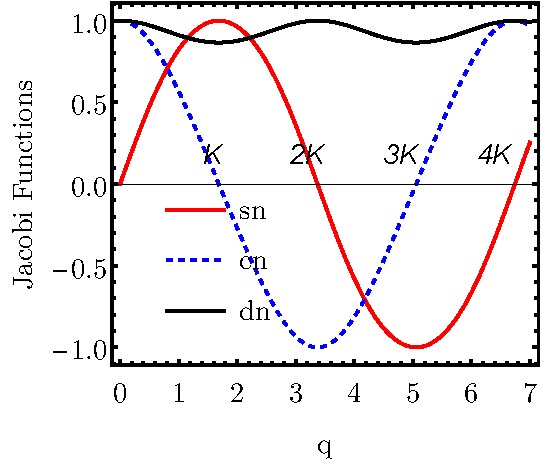
\includegraphics[scale=0.9]{Chapters/Figures/Jacobi-Elliptic-Functions.pdf}
    \caption{The elliptic functions sn, cd, and dn from Eq. \eqref{elliptic-functions-equation} are represented as functions of $q$. The value of the \emph{elliptic modulus} $k$ is set to $1/2$.}
    \label{elliptic-functions-plot}
\end{figure}

Referring back to the angular momentum components, these can be written in terms of the elliptic functions and the variables $q$, $d/dq$ as such \cite{raduta2020new}:
\begin{align}
    \hat{I}_\pm&=i\frac{c\mp d}{k's}\left(I\pm\hat{I}_0\right)\ ,\nonumber\\
    \hat{I}_0&=Icd-s\frac{d}{dq}\ ,
    \label{angular-momentum-elliptic-representation}
\end{align}
which would make the Hamiltonian $\hat{H}'$ from Eq. \eqref{hamiltonian-new-boson-ladder-operators} achieve the following shape:
\begin{align}
    \hat{H}'=-\frac{d^2}{dq^2}-2v_0s\frac{d}{dq}+I(I+1)s^2k^2+2v_0cdI\ .
    \label{boson-hamiltonian-complete-form}
\end{align}

By changing the wave-function $\ket{\Psi}$ to:
\begin{align}
    \ket{\Psi}=\left(d-kc\right)^{-\frac{v_0}{k}}\ket{\Phi}\ ,
\end{align}
the Schrödinger equation will have two fully separated \emph{kinetic} and \emph{potential} terms:
\begin{align}
    \left[-\frac{d^2}{dq^2}+V(q)\right]\ket{\Phi}=E\ket{\Phi}\ .
    \label{schrodinger-equation-elliptic}
\end{align}

The potential term $V(q)$ is defined as \cite{raduta2020new}:
\begin{align}
    V(q)=\left[I(I+1)k^2+v_0^2\right]s^2+\left(2I+1\right)v_0cd\ .
    \label{elliptic-potential-formula}
\end{align}
and it is graphically represented in Fig. \ref{elliptic-potential-plot}. It can be seen that $V(q)$ has a symmetry to the change of sign for the coordinate $q$. If the potential is calculated for the interval $q\in\left[-4K,4K\right]$, it has three deep symmetric wells, with degenerate minima, and two local minima surrounding $q=\pm 2K$. The states near the local minima are meta-stable, meaning that through a tunneling effect, they can transition to adjacent minima. These characteristics are illustrated in Fig. \ref{elliptic-potential-plot-deep-mininma}.
\begin{figure}
    \centering
    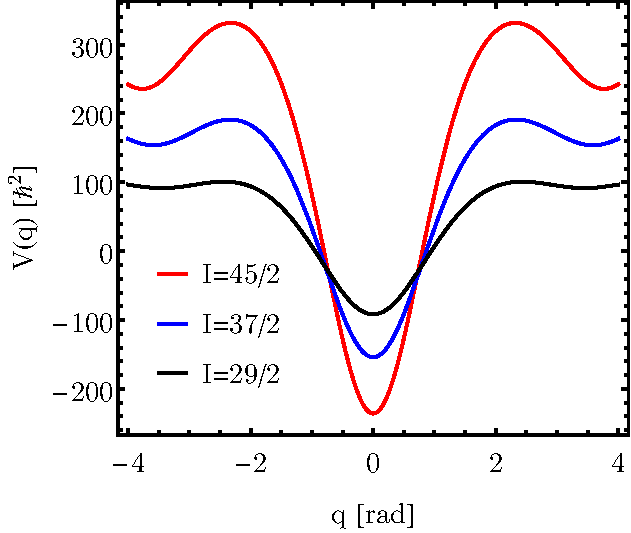
\includegraphics[scale=0.8]{Chapters/Figures/Elliptic-Potential-V.pdf}
    \caption{The potential energy as function of $q$ for several values of the angular momentum $I$. For the calculation of $V(q)$, the MOI were set to $\mathcal{I}_1:\mathcal{I}_2:\mathcal{I}_3=95:100:85\ \hbar\text{MeV}^{-2}$, $j=13/2$, and $\theta=-80^\circ$.}
    \label{elliptic-potential-plot}
\end{figure}
\begin{figure}
    \centering
    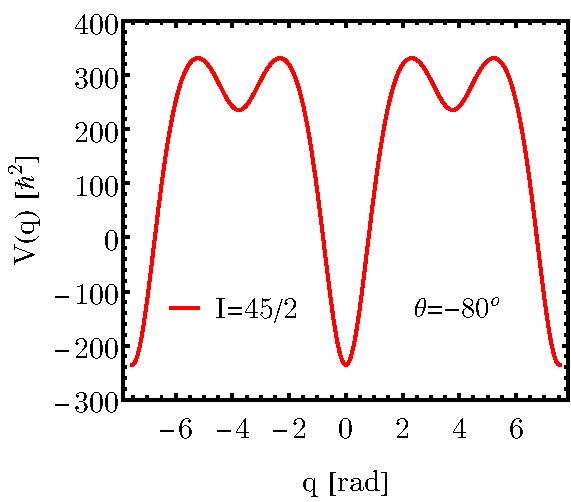
\includegraphics[width=0.49\textwidth]{Chapters/Figures/Elliptic-Potential-deep-1.pdf}
    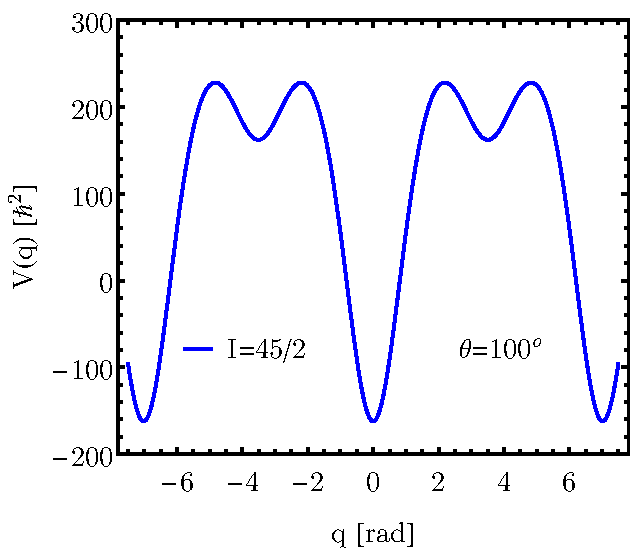
\includegraphics[width=0.49\textwidth]{Chapters/Figures/Elliptic-Potential-deep-1-180.pdf}
    \caption{The potential energy $V(q)$ for $\theta=-80^\circ$ and $\theta+\pi$, but for an extended range of the variable $q$, such that the deep and local minima can be seen. The same moments of inertia are used as in Fig. \ref{elliptic-functions-plot}.}
    \label{elliptic-potential-plot-deep-mininma}
\end{figure}

By adopting the Bargmann representation for the angular momentum representation depicted in Eq. \eqref{angular-momentum-elliptic-representation}, a set of boson operators for the variable $q$ and its first-derivative operator can be mapped:
\begin{align}
    q\rightarrow b^\dagger\ ,\ \frac{d}{dq}\rightarrow b\ ,
    \label{new-boson-bargmann-mapping}
\end{align}
and this results in the three components $\hat{I}_{\mp}$ and $\hat{I}_0$ becoming \cite{raduta2020new}:
\begin{align}
    \hat{I}_+&=\iu\frac{cb^\dagger-db^\dagger}{k'sb^\dagger}\left(I+Icb^\dagger db^\dagger-sb^\dagger b\right)\ ,\nonumber\\
    \hat{I}_-&=\iu\frac{cb^\dagger+db^\dagger}{k'sb^\dagger}\left(I-Icb^\dagger d b^\dagger+sb^\dagger b\right)\ ,\nonumber\\
    \hat{I}_0&=Icb^\dagger db^\dagger-sb^\dagger b\ .
    \label{angular-momentum-elliptic-bargmann}
\end{align}

\emph{This is the first time in literature when such a transformation emerges}. The remarkable features of the work presented in Ref. \cite{raduta2020new} are the boson expansion of angular momentum components obtained from elliptic functions $s$, $c$, and $d$, and the application of the Bargmann mapping depicted in Eq. \eqref{new-boson-bargmann-mapping} to these components.

\subsection{Another boson expansion for the angular momentum}

Particular attention should be paid to the case where $k=0$, as the elliptic functions will have the following values:
\begin{align}
    q=\varphi\ ,\ d=1\ , K=\frac{\pi}{2}\ ,\ k'=1\ .
\end{align}

Using these values, the components from Eq. \eqref{angular-momentum-elliptic-bargmann} can be re-written such that in the rotating frame they become:
\begin{align}
    \hat{I}_+&=\iu\left[-I\sin b^\dagger+\left(1-\cos b^\dagger\right)b^\dagger\right]\ ,\nonumber\\
    \hat{I}_-&=\iu\left[I\sin b^\dagger+\left(1+\cos b^\dagger\right)b\right]\ ,\nonumber\\
    \hat{I}_0&=I\cos b^\dagger-b\sin b^\dagger\ ,
    \label{angular-momentum-new-expansion}
\end{align}
which can be simplified even more if the trigonometric functions are expanded and only the leading terms are kept:
\begin{align}
    \hat{I}_+&=\iu\left[-Ib^\dagger+\frac{1}{2}b\left(b^\dagger\right)^2\right]\ ,\nonumber\\
    \hat{I}_-&=2\iu b\ ,\nonumber\\
    \hat{I}_0&=I-b^\dagger b\ .
    \label{angular-momentum-dyson-expansion}
\end{align}

The components from Eq. \eqref{angular-momentum-dyson-expansion} are similar to the ones from the Dyson boson expansion (recall Eq. \eqref{dyson-transformation}), making it clear now that the representations shown in Eq. \eqref{angular-momentum-elliptic-bargmann} and Eq. \eqref{angular-momentum-new-expansion} are generalizations of the Dyson representation.

\subsection{Harmonic Approximation of the Energy}

One can aim at solving numerically Eq. \eqref{schrodinger-equation-elliptic}, but there could be a rather simpler and more \emph{elegant} approach to this. Adopting the harmonic approximation (as described in the previous chapters) can provide valid results. The first step is to analyze the stationary points of the elliptic potential $V(q)$. Its first-order derivative is given by \cite{raduta2020new}:
\begin{align}
    \frac{d}{dq}V(q)=s\left[\left(I(I+1)k^2+v_0^2\right)2cd-(2I+1)v_0k'^2-(2I+1)v_02k^2c^2\right]\ .
\end{align}

There are five minima, located at $q=0,\pm2K,\pm4K$. Remarkable that for $q=\pm2K$ the two minima emerge for angular momentum values that are larger than $19/2$. This is emphasized in Fig. \ref{elliptic-potential-plot-2k-minima}, where it can be seen that the minima are flat at the beginning, but their depth increases with increasing values of $I$.
\begin{figure}
    \centering
    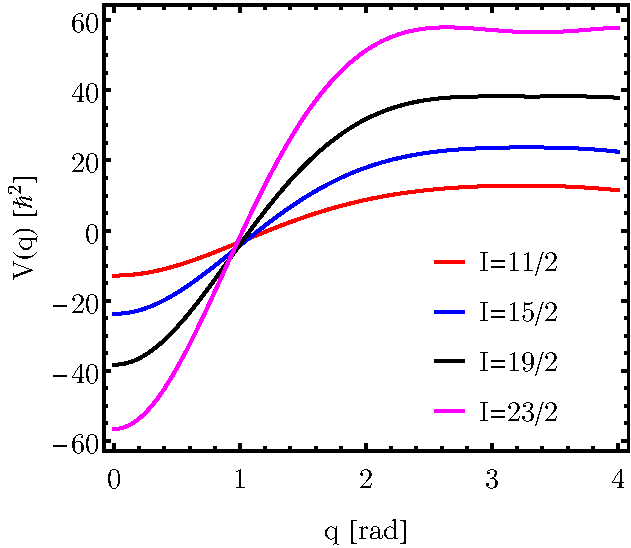
\includegraphics[scale=0.8]{Chapters/Figures/Elliptic-Potential-2K-Minima.pdf}
    \caption{The potential $V(q)$ from Eq. \eqref{elliptic-potential-formula}, near the $q=2K$ minimum point. It can be observed that the minimum character appears only for $I>19/2$.}
    \label{elliptic-potential-plot-2k-minima}
\end{figure}

The angular momentum can be studied in terms of its orientation near the minimum points. This is achieved if the boson expansion is written as \cite{raduta2020new}:
\begin{align}
    \hat{I}_+&=\frac{\iu}{k'}\left[I\left(-d+ck^2\right)s-(c-d)\frac{d}{dq}\right]\ ,\nonumber\\
    \hat{I}_-&=\frac{\iu}{k'}\left[I\left(d+ck^2\right)s+(c+d)\frac{d}{dq}\right]\ ,\nonumber\\
    \hat{I}_0&=Icd-s\frac{d}{dq}\ ,
\end{align}
and for $q=\pm2K$ (that is $\varphi=\pm\pi$) one has $\hat{I}_0=-I$, while $q=0$ (i.e., $\varphi=2$) will lead to $\hat{I}_0=I$. Consequently, in the local minima, the total angular momentum will align anti-parallel with the $1$-axis, and for the deep minimum $q=0$ the angular momentum is aligned along the (1)-axis. Expanding the elliptic potential $V(q)$ up to second order in the coordinate, an equation that looks similar to the harmonic oscillator is obtained for the Hamiltonian $\hat{H}_\text{rot}$ (firstly introduced in Eq. \eqref{rotor-hamiltonian-new-boson}):
\begin{align}
    E_n=A_1I^2+\hbar\omega\left(n+\frac{1}{2}\right)+e_\text{sp}\ ,
    \label{energy-2nd-order-expansion-deepest-minima}
\end{align}
where the single-particle term is defined as:
\begin{align}
    e_\text{sp}=\sum_{i=1,2}A_ij_i^2-(2I+1)A_1j_1-IA_2j_2\ .
\end{align}

The frequency $\omega$ from Eq. \eqref{energy-2nd-order-expansion-deepest-minima} has the expression:
\begin{align}
    \omega^2=&\left[(2I+1)\left(A_2-A_1-\frac{A_2j_2}{I}\right)+2A_1j_1\right]\cdot\nonumber\\
    &\cdot\left[(2I+1)(A_3-A_1)+2A_1j_1\right]-(A_3-A_1)\left(A_2-A_1-\frac{A_2j_2}{I}\right)\ .
    \label{omega-frequency-deepest-minima}
\end{align}

% On the other hand, if the potential is expanded around the local minimum $q=2K$, and only the quadratic terms are kept, then the following set of energies :
% \begin{align}
    %     E_n^{(2K)}&=-(2I+1)v_0+\hbar\omega^{(2K)}\left(n+\frac{1}{2}\right)\ ,\nonumber\\
    %     \left(\omega^{(2K)}\right)^2&=\left(1+\frac{2v_0}{2I+1}\right)\left(u+\frac{2v_0}{2I+1}\right)(2I+1)^2-u\ ,
    % \end{align}
    
    The Hamiltonian $\hat{H}_\text{rot}$ is connected to $\hat{H}'$ via Eq. \eqref{rewritten-rotor-hamiltonian-new-boson}, meaning that the final energy spectrum of $\hat{H}'$ will be given by:
    \begin{align}
        E_n'&=A_1I^2+\hbar\omega'\left(n+\frac{1}{2}\right)+e_\text{sp}\ ,\nonumber\\
        e_\text{sp}&=\sum_{i=1,2}A_ij_i^2-(2I+1)A_1j_1-IA_2j_2\ ,
        \label{energy-2nd-order-expansion-local-minima}
\end{align}
with the wobbling frequency $\omega'$ having the following definition:
\begin{align}
    \omega'^2=&\left[(2I+1)\left(A_2-A_1-\frac{A_2j_2}{I}\right)-2A_1j_1\right]\left[(2I+1)(A_3-A_1)-2A_1j_1\right]-\nonumber\\
    &-(A_3-A_1)\left(A_2-A_1-\frac{A_2j_2}{I}\right)
    \label{wobbling-frequency-new-boson-prime}
\end{align}

The two wobbling frequencies, i.e., $\omega$ and $\omega'$ are both graphically represented in Fig. \ref{wobbling-frequencies-harmonic-approx}. As the angular momentum components $j_1$ and $j_2$ depend on the angle $\theta$, the evolution of both frequencies is plotted as a function of this coordinate. It can be seen from the two curves that both wobbling frequencies have a maximum value $\approx1$, but $\omega_\text{max}$ is located at $\theta\approx-0.7\ \text{rad}$, while $\omega'_\text{max}$ is at $\theta\approx-2.4\ \text{rad}$. Moreover, the two frequencies intersect each other at the points $\theta=-\pi/2$ and $\theta=\pi/2$.
\begin{figure}
    \centering
    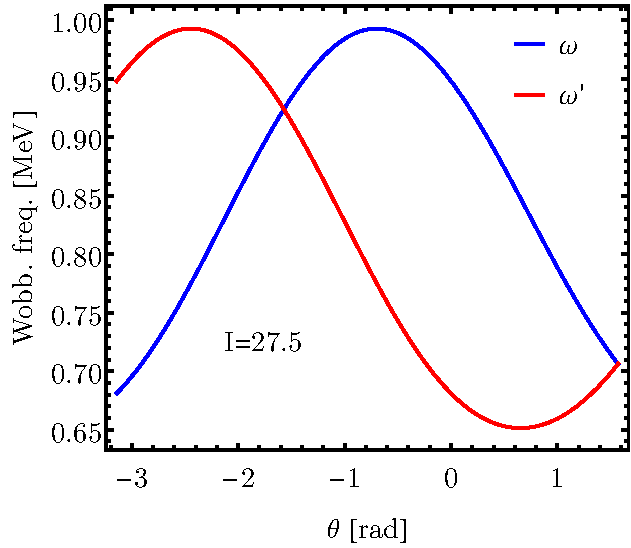
\includegraphics[scale=0.8]{Chapters/Figures/Wobbling-Frequencies-New-Boson.pdf}
    \caption{The two wobbling frequencies $\omega$ (Eq. \eqref{omega-frequency-deepest-minima}) and $\omega'$ (Eq. \eqref{wobbling-frequency-new-boson-prime}) as function of the coordinate $\theta$ for a fixed set of MOI $\mathcal{I}_1:\mathcal{I}_2:\mathcal{I}_3=91:9:51\ \hbar^2\text{MeV}^{-1}$ and single-particle angular momentum $j=13/2$.}
    \label{wobbling-frequencies-harmonic-approx}
\end{figure}

\section{Classical Description of the Hamiltonian}
\label{classical-description-new-boson-section}

Going further with the analysis performed in Ref. \cite{raduta2020new}, the quantal operators associated with the angular momentum are dequantized, through the algebra:
\begin{align}
    [\ ,\ ] \longrightarrow -\iu\{\ ,\ \}\ ,
\end{align}
where the Poisson brackets replace the commutator. The dequantization procedure consists of replacing the operators $\hat{I}_k$ with the classical components of the angular momentum $I_k$. The conjugate coordinate of $I_k$ are further denoted by $\varphi_k$ and the three angular momentum components $I_k$ are hereafter denoted by $x_k$. With this algebra, the quantal Hamiltonian from Eq. \eqref{new-boson-hamiltonian-notations} will be equivalent to:
\begin{align}
    H'=x_2^2+ux_3^2+2v_0I_x\ .
    \label{new-boson-h-prime-classical}
\end{align}

Such an approach was also used when studying the Classical Energy Function (CEF) from Chapter \ref{chapter-5-novel} (recall Eq. \eqref{polar-coordinates-total-AM}). The equations of motion for $H'$ are (time derivatives are specified by the dot symbol):
\begin{align}
    \dot{x}_1&=2(1-u)x_2x_3\ ,\nonumber\\
    \dot{x}_2&=2(x_1u-v_0)x_3\ ,\nonumber\\
    \dot{x}_3&=-2(x_1-v_0)x_2\ .
\end{align}

The two constants of motion for this classical problem are:
\begin{align}
    E=x_2^2+ux_3^2+2v_0x_1\ ,
\end{align}
and:
\begin{align}
    I^2=x_1^2+x_2^2+x_3^2\ ,
\end{align}
which is in complete agreement with the fact the total energy and the total angular momentum are conserved quantities. Now that the classical counterpart of $\hat{H}'$ is analytically obtained, there can be several situations that can lead to the description of the harmonic-like motion of the even-odd system. Namely, by considering the three angular momentum components $x_1$, $x_2$, and $x_3$ in the \emph{polar coordinate system} (defined by the coordinates $\theta$ and $\varphi$), one can have multiple considerations.

\subsubsection*{Case A1}

The maximal MOI corresponds to the $2$-axis. The Cartesian coordinates are changed to the polar ones via:
\begin{align}
    x_2=I\cos\theta_2\ ,\ x_3=I\sin\theta_2\cos\varphi_2\ ,\ x_1=I\sin\theta_2\sin\varphi_2\ .
    \label{polar-coordinates-case-a1}
\end{align}

The energy function $H'$ can be expressed in terms of the conjugate coordinates $(x_2,\varphi_2)$:
\begin{align}
    H'=x_2^2\left(1-u\cos^2\varphi_2-\frac{v_0}{I}\sin\varphi_2\right)+uI^2\cos^2\varphi_2+2v_0I\sin\varphi_2\ .
    \label{classical-energy-new-boson-2-axis}
\end{align}
This function has a minimum value of $H'\vert_\text{min}=-2v_0I$ at $(x_2,\varphi_2)=(0,-\pi/2)$, and the second derivatives for $H'$ in that point are:
\begin{align}
    \left.\frac{\partial^2H'}{\partial x_2^2}\right\vert_\text{min}&=2\left(2+\frac{v_0}{I}\right)\ ,\nonumber\\
    \left.\frac{\partial^2 H'}{\partial \varphi_2^2}\right\vert_\text{min}&=2\left(u+\frac{v_0}{I}\right)I^2\ .
\end{align}

If the classical energy function is expanded up to the second order around the minimum point, then $H'$ will look like this:
\begin{align}
    H'^{(2)}=-2v_0I\left(1+\frac{v_0}{I}\right)\bar{x}_2^2+\left(u+\frac{v_0}{I}\right)I^2\bar{\varphi}_2^2\ ,
\end{align}
where the deviation of the coordinates from the minimum point was denoted by $(\bar{x}_2,\bar{\varphi}_2)$ and the superscript $(2)$ suggests the second order expansion. This kind of function describes an oscillator with the frequency:
\begin{align}
    \omega^{(2)}=2\sqrt{(I+v_0)(Iu+v_0)}\ .
\end{align}

In the minimum point, the angular momentum components are $(x_1,x_2,x_3)=(-I,0,0)$ and $E=-2v_0I$. In Fig. \ref{energy-function-comparison-a1-case} the energy function $H'$ is graphically represented for $x_2=0$ and $\varphi_2=-\pi/2$, respectively, by keeping one coordinate fixed and varying the other. On both plots, the minimum value for $H'$ is achieved at the value $-2Iv_0$.
\begin{figure}
    \centering
    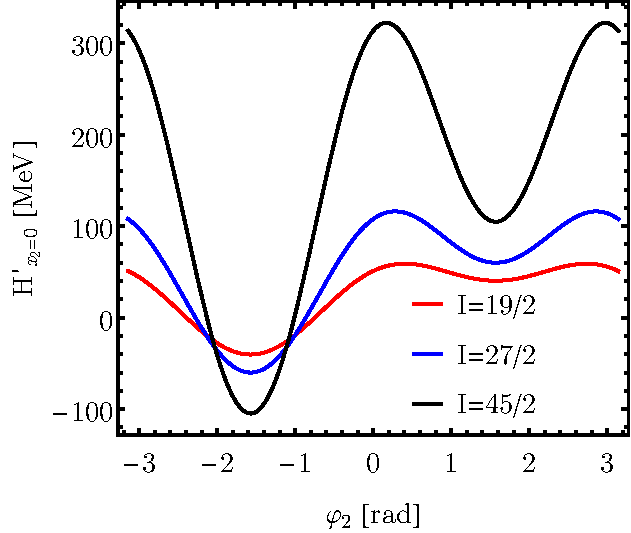
\includegraphics[width=0.49\textwidth]{Chapters/Figures/Energy-Function-New-Boson-A1-x2-const.pdf}
    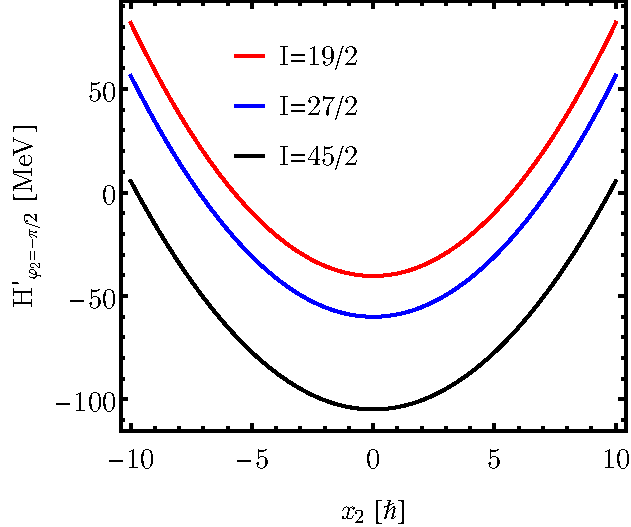
\includegraphics[width=0.49\textwidth]{Chapters/Figures/Energy-Function-New-Boson-A1-phi2-const.pdf}
    \caption{The classical energy $H'$ from Eq. \eqref{classical-energy-new-boson-2-axis} evaluated for a fixed $x_2=0$ (left) and fixed $\varphi_2=-\pi/2$ (right). The calculations were done for $\mathcal{I}_1:\mathcal{I}_2:\mathcal{I}_3=10:40:20\ \hbar\text{MeV}^{-1}$. The single-particle angular momentum $j=11/2$.}
    \label{energy-function-comparison-a1-case}
\end{figure}

\subsubsection*{Case A2}

Another minimum point for $H'$ is $(0,\pi/2)$, in which the angular momentum is $(x_1,x_2,x_3)=(I,0,0)$ and the energy is $E=2v_0I$. Repeating the second order expansion for $H'$, the following formula is attained:
\begin{align}
    H'^{(2)}=2v_0I+\left(1-\frac{v_0}{I}\right)\bar{x}_2^2+I^2\left(u-\frac{v_0}{I}\right)\bar{\varphi}_2^2\ ,
\end{align}
which describes a harmonic oscillator with a frequency:
\begin{align}
    % \omega^{(2)}=2\sqrt{\left(1-\frac{v_0}{I}\right)\left(u-\frac{v_0}{I}\right)I^2}\ .
    \omega^{(2)}=2\sqrt{(I-v_0)(uI-v_0)}\ .
\end{align}

\subsubsection*{Case A3}

A third set of conjugate variables for which $H'$ is minimal is: $$(x_2,\varphi_2)=(0,\arcsin\left(\frac{v_0}{Iu}\right))\ .$$ With this set of coordinates the energy function will become after expansion:
\begin{align}
    H'^{(2)}=uI^2+\frac{v_0^2}{u}+(1-u)\bar{x}_2^2-u\left(I^2-\frac{v_0^2}{u^2}\right)\bar{\varphi}_2^2\ .
\end{align}

For a positive value of $u$, but confined inside $u\in(0,1)$ the coordinates consist of a \emph{saddle point} with angular momentum components: $$(x_1,x_2,x_3)=\left(\frac{v_0}{u},0,\sqrt{I^2-\frac{v_0^2}{u^2}}\right)\ ,$$ and energy: $$E=I^2u+\frac{v_0^2}{u}\ .$$

Summarizing the situations $A1$, $A2$, and $A3$, there are three stationary points for $H'$ when the maximal MOI is along the $2$-axis, (i.e., the quantization axis). The points are provided in Table \ref{stationary-points-2-axis}, where values for $x_2$ and $\varphi_2$ are accompanied by the angular momentum components and the value of the energy. Moreover, the character of each stationary point is also mentioned.
\begin{table}
    \centering
    \caption{The stationary points for the classical energy function depicted in Eq. \eqref{new-boson-h-prime-classical}, when the quantization axis is the $2$-axis. Each point corresponds to the cases $A1$, $A2$, and $A3$, respectively.}
    \resizebox{\textwidth}{!}{%
    \begin{tabular}{cccccc}
    \hline
    \multicolumn{1}{c}{Point $p$} &
    \multicolumn{1}{c}{$x_2$} &
    \multicolumn{1}{c}{$\varphi_2$} &
    \multicolumn{1}{c}{\begin{tabular}[c]{@{}c@{}}A.m. components\\ $(x_1,x_2,x_3)$\end{tabular}} &
    \multicolumn{1}{c}{$E$} &
    \multicolumn{1}{c}{\begin{tabular}[c]{@{}c@{}}Character \\ of the stationary point\end{tabular}} \\ \hline \hline
    $p_1^A(m)$ & $0$ &  $-\frac{\pi}{2}$    & $(-I,0,0)$ & $E=-2v_0I$ & minimum (m) \\
    $p_2^A(m)$ & $0$ &  $\frac{\pi}{2}$    & $(I,0,0)$ & $E=2v_0I$ & minimum (m) \\
    $p_3^A(s)$ & $0$ &  $\arcsin\left(\frac{v_0}{Iu}\right)$  & $\left(\frac{v_0}{u},0,\sqrt{I^2-\frac{v_0^2}{u^2}}\right)$ & $E=\left(I^2u+\frac{v_0^2}{u}\right)$ & saddle (s)\\
    \hline
    \end{tabular}%
    }
    \label{stationary-points-2-axis}
\end{table}

Considering that the polar coordinates used to define the three angular momentum components can be replaced in the expression of $H'$ from Eq. \eqref{new-boson-h-prime-classical}, then an energy function that will depend explicitly on $\theta_2$ and $\varphi_2$. This \emph{polar representation of the classical energy function} can be represented for a given interval of $\theta_2$ and $\varphi_2$, respectively. Fixing the total angular momentum $I$, the single-particle a.m. $j$, the three MOI, and the value of $\theta$ (not to be confused with the polar $\theta_2$), a contour plot such as the one shown in Fig. \ref{new-boson-hprime-2axis-contour-plot} can be obtained. Within the contour plot, there are several stationary points: one deep minimum, one local minimum, and two saddle points. Every point lies along the $\theta_2=\pi/2$ coordinate. To better perceive how the minima and saddle points are located, Fig. \ref{new-boson-hprime-2axis-varphi-plot} shows the evolution of $H'$ for $\theta_2=\pi/2$. Keep in mind that both figures are evaluated for the same set of constants.
\begin{figure}
    \begin{center}
        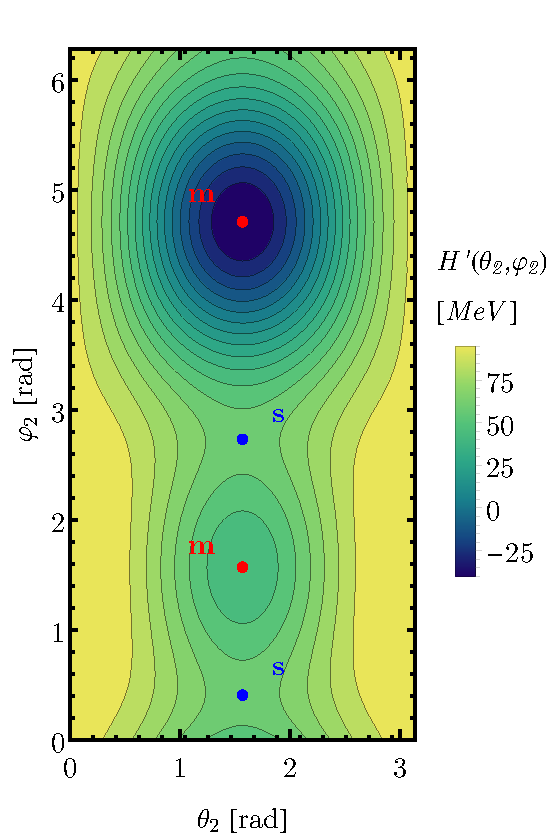
\includegraphics[scale=0.7]{Chapters/Figures/New-Boson-Classical-H-2axis-quantization.pdf}
        \caption{Contour plot for the energy $H'$ from Eq. \eqref{new-boson-h-prime-classical}, defined in terms of the polar coordinates. The calculations are done for the A1-A2-A3 cases (i.e., maximal MOI is $\mathcal{I}_2)$. The single-particle angular momentum is $j=11/2$, the total angular momentum $I=19/2$, the MOI are $\mathcal{I}_1:\mathcal{I}_2:\mathcal{I}_3=10:40:20\ \hbar^2\text{MeV}^{-1}$, and $\theta=70^\circ$. The four stationary points are illustrated, namely two minima - one local and one global - (denoted by "m") and two saddle points (denoted by "s").}
        \label{new-boson-hprime-2axis-contour-plot}
    \end{center}
\end{figure}
\begin{figure}
    \begin{center}
        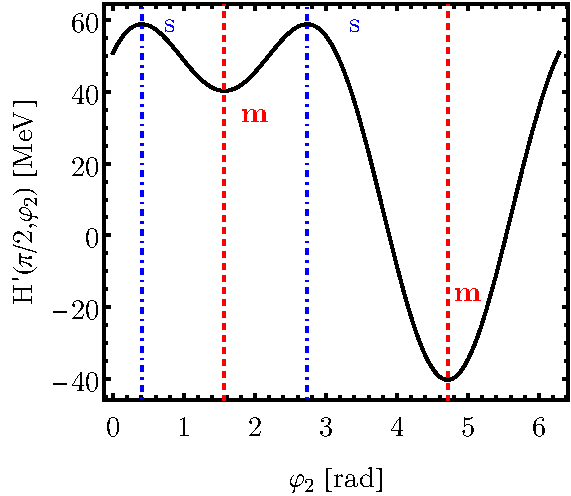
\includegraphics[scale=0.8]{Chapters/Figures/New-Boson-Classical-H-2-axis-varphi-plot.pdf}
        \caption{The classical energy $H'$ from Eq. \eqref{new-boson-h-prime-classical}, for a fixed $\theta_2=\pi/2$ and $\varphi\in[0,2\pi]$. The single-particle angular momentum is $j=11/2$, the total angular momentum $I=19/2$, the MOI are $\mathcal{I}_1:\mathcal{I}_2:\mathcal{I}_3=10:40:20\ \hbar^2\text{MeV}^{-1}$, and $\theta=70^\circ$. The critical points present in Fig. \ref{new-boson-hprime-2axis-contour-plot} are also illustrated here by the dashed vertical lines (two minima with red color and two saddle points with blue color).}
        \label{new-boson-hprime-2axis-varphi-plot}
    \end{center}
\end{figure}

\subsubsection*{Case B1}

Going further with the analysis, a second approach would be to consider the $3$-axis as the quantization axes, meaning that now the largest MOI is around this axis. The angular momentum components written in terms of the polar coordinates $(\theta_3,\varphi_3)$ will be defined in the following way:
\begin{align}
    x_1=I\sin\theta_3\cos\varphi_3\ ,\ x_2=I\sin\theta_3\sin\varphi_3\ ,\ x_3=I\cos\theta_3\ ,
    \label{polar-coordinates-case-b1}
\end{align}

In the same way as the $A$-cases. the total energy $H'$ can be expressed in terms of the $x_3$ coordinate and the polar $\varphi_3$ one:
\begin{align}
    H'^{(2)}=x_3^2\left(u-\sin^2\varphi_3-\frac{v_0}{I}\cos\varphi_3\right)+I^2\sin^2\varphi_3+2v_0I\cos\varphi_3\ .
    \label{classical-energy-new-boson-3-axis}
\end{align}

The first stationary point of Eq. \eqref{classical-energy-new-boson-3-axis} with a minimum character is $(x_3,\varphi_3)=(0,\pi)$. For this point, the angular momentum components are $(x_1,x_2,x_3)=(-I,0,0)$, hinting at the fact that the total a.m. is oriented along the one-axis. The value of the energy in this point is $E=-2v_0I$. The harmonic Hamiltonian given in the second-order expansion around this point is:
\begin{align}
    H'^{(2)}=-2v_0I+\left(u+\frac{v_0}{I}\right)\bar{x}_3^2+I^2\left(1+\frac{v_0}{I}\right)\bar{\varphi}_3^2\ ,
\end{align}

having a similar shape for the wobbling frequency as per the $A1$ case. Similarly as for the $A1$ case, the Hamiltonian $H'$ is also represented in terms of only one coordinate at a time, where each of the coordinates is fixed to $x_3=0$ and $\varphi_3=\pi$, respectively. These plots are shown in Figs. \ref{energy-function-comparison-b1-case}.
\begin{figure}
    \centering
    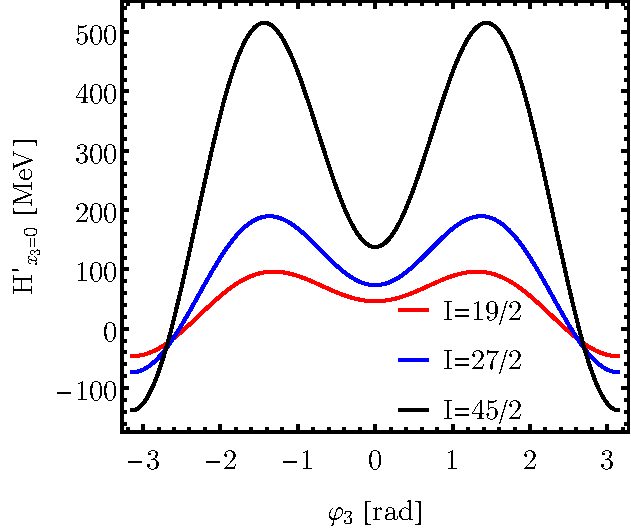
\includegraphics[width=0.49\textwidth]{Chapters/Figures/Energy-Function-New-Boson-B1-x3-const.pdf}
    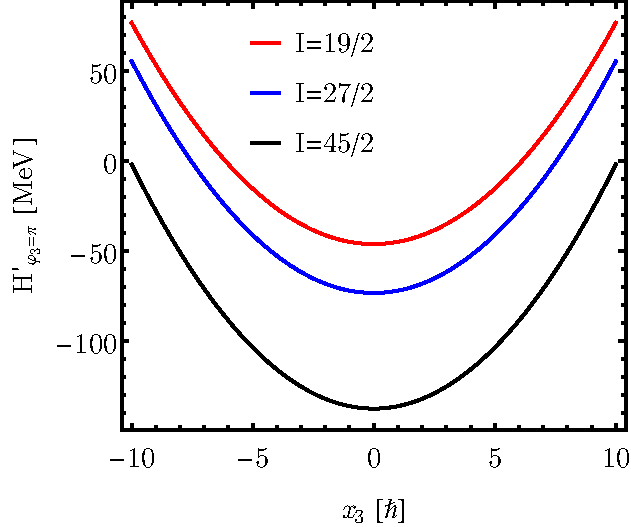
\includegraphics[width=0.49\textwidth]{Chapters/Figures/Energy-Function-New-Boson-B1-phi3-const.pdf}
    \caption{The classical energy $H'$ from Eq. \eqref{classical-energy-new-boson-3-axis} evaluated for a fixed $x_3=0$ (left) and fixed $\varphi_3=\pi$ (right). The calculations were done for $\mathcal{I}_1:\mathcal{I}_2:\mathcal{I}_3=10:20:40\ \hbar^2\text{MeV}^{-1}$. The single-particle angular momentum $j=11/2$.}
    \label{energy-function-comparison-b1-case}
\end{figure}

\subsubsection*{B2 case}

Another stationary point for Eq. \eqref{classical-energy-new-boson-3-axis} is $(x_3,\varphi)=(0,0)$, which is also a minimum. The second order expansion of $H'$ gives:
\begin{align}
    H'=2v_0I+\left(u-\frac{v_0}{I}\right)\bar{x}_3^2+I^2\left(1-\frac{v_0}{I}\right)\bar{\varphi}_3^2\ ,
\end{align}
and moreover $(x_1,x_2,x_3)=(I,0,0)$, and $E=2v_0I$. The wobbling frequency is:
\begin{align}
    \omega^{(2)}=2\sqrt{\left(1-\frac{v_0}{I}\right)\left(u-\frac{v_0}{I}\right)I^2}\ .
\end{align}

\subsubsection*{B3 case}

Lastly, the stationary point $(x_3,\varphi_3)=\left(0,\arccos\frac{v_0}{I}\right)$ is a maximum, giving a.m. components:
\begin{align}
    (x_1,x_2,x_3)=\left(v_0,\sqrt{I^2-v_0^2},0\right)\ ,
\end{align}
and energy $E=I^2+v_0^2\ .$ For this maximum point, the energy function $H'$ becomes:
\begin{align}
    H'^{(2)}=I^2+v_0^2+\left(u-1\right)\bar{x}_3^2+\left(v_0^2-I^2\right)\bar{\varphi}_3^2\ .
\end{align}

The contour plot of the energy function $H'$ can be obtained in the same manner as for $A$ situations, i.e., taking the polar coordinates $(\theta_3,\varphi_3)$ that are used in the expression of the angular momentum components from Eq. \eqref{polar-coordinates-case-b1}, and evaluate $H'(\theta_3,\varphi_3)$ for fixed values of $j,\ I,\ \mathcal{I}_1,\ \mathcal{I}_2,\ \mathcal{I}_3$, and $\theta$. The contour plot together with the evolution of $H'(\pi,\varphi_3)$ are drawn in Figs. \ref{new-boson-hprime-3axis-contour-plot} - \ref{new-boson-hprime-3axis-varphi-plot}.
\begin{figure}
    \begin{center}
        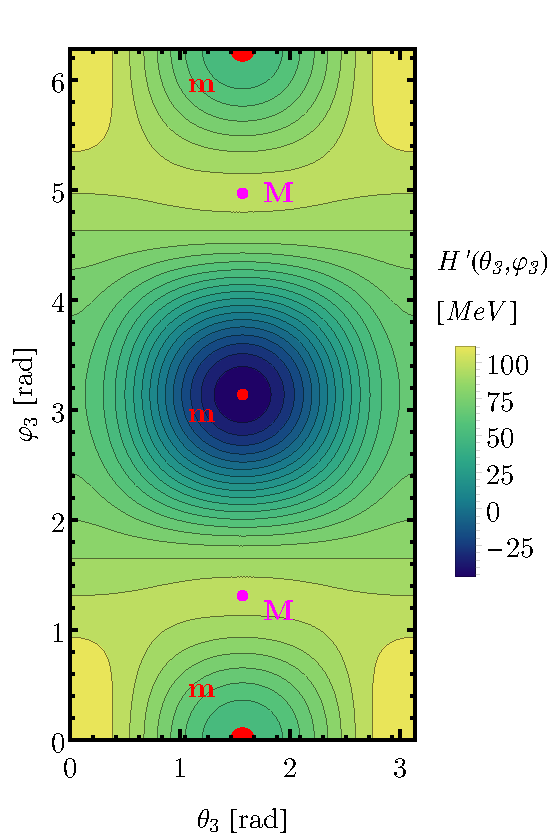
\includegraphics[scale=0.7]{Chapters/Figures/New-Boson-Classical-H-3axis-quantization.pdf}
        \caption{Contour plot for the energy $H'$ from Eq. \eqref{new-boson-h-prime-classical}, defined in terms of the polar coordinates. The calculations are done for the B1-B2-B3 cases (i.e., maximal MOI is $\mathcal{I}_3)$. The single-particle angular momentum is $j=11/2$, the total angular momentum $I=19/2$, the MOI are $\mathcal{I}_1:\mathcal{I}_2:\mathcal{I}_3=10:20:40\ \hbar^2\text{MeV}^{-1}$, and $\theta=70^\circ$. The five stationary points are illustrated, namely two maxima (denoted by "M") and three minimum points (denoted by "m"; one global and two local).}
        \label{new-boson-hprime-3axis-contour-plot}
    \end{center}
\end{figure}
\begin{figure}
    \begin{center}
        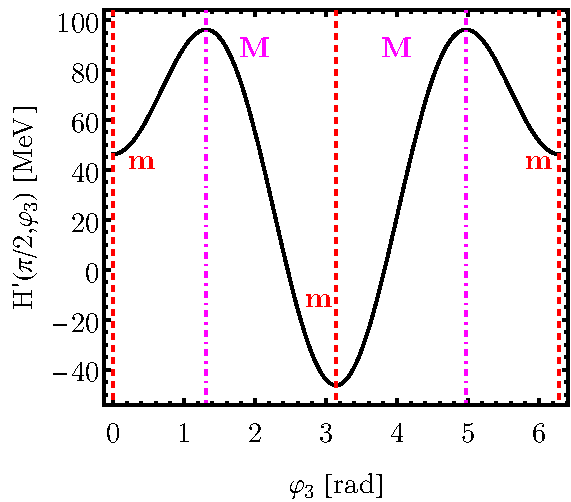
\includegraphics[scale=0.8]{Chapters/Figures/New-Boson-Classical-H-3-axis-varphi-plot.pdf}
        \caption{The classical energy $H'$ from Eq. \eqref{new-boson-h-prime-classical}, for a fixed $\theta_2=\pi/2$ and $\varphi\in[0,2\pi]$. The single-particle angular momentum is $j=11/2$, the total angular momentum $I=19/2$, the MOI are $\mathcal{I}_1:\mathcal{I}_2:\mathcal{I}_3=10:20:40\ \hbar^2\text{MeV}^{-1}$, and $\theta=70^\circ$. The critical points present in Fig. \ref{new-boson-hprime-3axis-contour-plot} are illustrated by the dashed vertical lines (magenta for the maxima and red for the minima).}
        \label{new-boson-hprime-3axis-varphi-plot}
    \end{center}
\end{figure}

Analyzing the Figs. \ref{new-boson-hprime-3axis-contour-plot} -\ref{new-boson-hprime-3axis-varphi-plot}, five stationary points can be observed: two maxima denoted by "M" (magenta color) and three minima denoted by "m" (red color). All the stationary points for the B cases are identified in Table \ref{stationary-points-3-axis}, similarity as for the A situations.
\begin{table}
    \centering
    \caption{The stationary points for the classical energy function depicted in Eq. \eqref{new-boson-h-prime-classical}, when the quantization axis is the $3$-axis. Each point corresponds to the cases $B1$, $B2$, and $B3$, respectively.}
    \resizebox{\textwidth}{!}{%
    \begin{tabular}{cccccc}
    \hline
    \multicolumn{1}{c}{Point $p$} &
    \multicolumn{1}{c}{$x_3$} &
    \multicolumn{1}{c}{$\varphi_3$} &
    \multicolumn{1}{c}{\begin{tabular}[c]{@{}c@{}}A.m. components\\ $(x_1,x_2,x_3)$\end{tabular}} &
    \multicolumn{1}{c}{$E$} &
    \multicolumn{1}{c}{\begin{tabular}[c]{@{}c@{}}Character \\ of the stationary point\end{tabular}} \\ \hline \hline
    $p_1^B(m)$ & $0$ &  $\pi$    & $(-I,0,0)$ & $E=-2v_0I$ & minimum (m) \\
    $p_2^B(m)$ & $0$ &  $0$    & $(I,0,0)$ & $E=2v_0I$ & minimum (m) \\
    $p_3^B(M)$ & $0$ &  $\arccos\left(\frac{v_0}{I}\right)$  & $\left(v_0,\sqrt{I^2-v_0^2},0\right)$ & $E=I^2\left(1+v^2\right)$ & maximum (M)\\
    \hline
    \end{tabular}%
    }
    \label{stationary-points-3-axis}
\end{table}

\subsubsection*{Case C1}

Lastly, the situation when the largest MOI corresponds to the $1$-axis should be analyzed. Choosing the $1$-axis as the quantization axis, the a.m. components are expressed in terms of the polar coordinates:
\begin{align}
    x_1=I\cos\theta_1\ ,\ x_2=I\sin\theta_1\cos\varphi_1\ ,\ x_3=I\sin\theta_1\sin\varphi_1,
    \label{polar-coordinates-case-c1}
\end{align}
with the associated Hamiltonian:
\begin{align}
    H'=\left(I^2-x_1^2\right)\left(\cos^2\varphi_1+u\sin^2\varphi_1\right)+2v_0x_1\ .
    \label{classical-energy-new-boson-1-axis}
\end{align}

The Hamiltonian from Eq. \eqref{classical-energy-new-boson-1-axis} has a stationary point at $(x_1,\varphi_1)=\left(\frac{v_0}{u},\frac{\pi}{2}\right)$. This is a \emph{saddle} point when $u\in(0,1)$. The second order expansion of $H'$ is therefore:
\begin{align}
    H'^{(2)}=uI+\frac{v_0}{u}-u\bar{x}_1^2+(1-u)\left(I^2-\frac{v_0^2}{u^2}\right)\bar{\varphi}_1^2\ .
\end{align}

\subsubsection*{Case C2}

Another stationary point for $H'$ is $(v_0,0)$, which has a maximum character, giving angular momentum components $(x_1,x_2,x_3)=(v_0,\sqrt{I^2-v_0},0)$ and $E=I^2+v_0^2\ .$ The second order expansion of the energy function is:
\begin{align}
    H'^{(2)}=I^2+v_0-\bar{x}_1^2(u-1)\left(I^2-v_0^2\right)\bar{\varphi}_1^2\ .
\end{align}

Similarly as in cases A-B, a contour plot showing the behavior of the energy function $H'$ would be useful. This is shown in Fig. \ref{new-boson-hprime-1axis-contour-plot}, where the calculation of $H'(\theta_1,\varphi_1)$ used a different set of MOI, namely: $\mathcal{I}_1:\mathcal{I}_2:\mathcal{I}_3=80:10:50\ \hbar^2\text{MeV}^{-1}$. The maxima from Fig \ref{new-boson-hprime-1axis-contour-plot} would illustrate that a rotation around the $1$-axis (the cranking axis for the initial system) is not possible. The critical points for the C cases are recorded in Table \ref{stationary-points-1-axis}.
\begin{table}
    \centering
    \caption{The stationary points for the classical energy function depicted in Eq. \eqref{new-boson-h-prime-classical}, when the quantization axis is the $1$-axis. Each point corresponds to the cases $C1$, and $C2$, respectively.}
    \resizebox{\textwidth}{!}{%
    \begin{tabular}{cccccc}
    \hline
    \multicolumn{1}{c}{Point $p$} &
    \multicolumn{1}{c}{$x_1$} &
    \multicolumn{1}{c}{$\varphi_1$} &
    \multicolumn{1}{c}{\begin{tabular}[c]{@{}c@{}}A.m. components\\ $(x_1,x_2,x_3)$\end{tabular}} &
    \multicolumn{1}{c}{$E$} &
    \multicolumn{1}{c}{\begin{tabular}[c]{@{}c@{}}Character \\ of the stationary point\end{tabular}} \\ \hline \hline
    $p_1^C(s)$ & $0$ &  $\pi$    & $\left(\frac{v_0}{u},0,\sqrt{\left(I^2-\frac{v_0^2}{u}\right)}\right)$ & $E=I^2u+\frac{v_0^2}{u}$ & saddle (s) \\
    $p_2^C(M)$ & $v_0$ &  $0$    & $\left(v_0,\sqrt{I^2-v_0^2},0\right)$ & $E=I^2+v_0^2$ & maximum (M) \\
    \hline
    \end{tabular}%
    }
    \label{stationary-points-1-axis}
\end{table}

\begin{figure}
    \begin{center}
        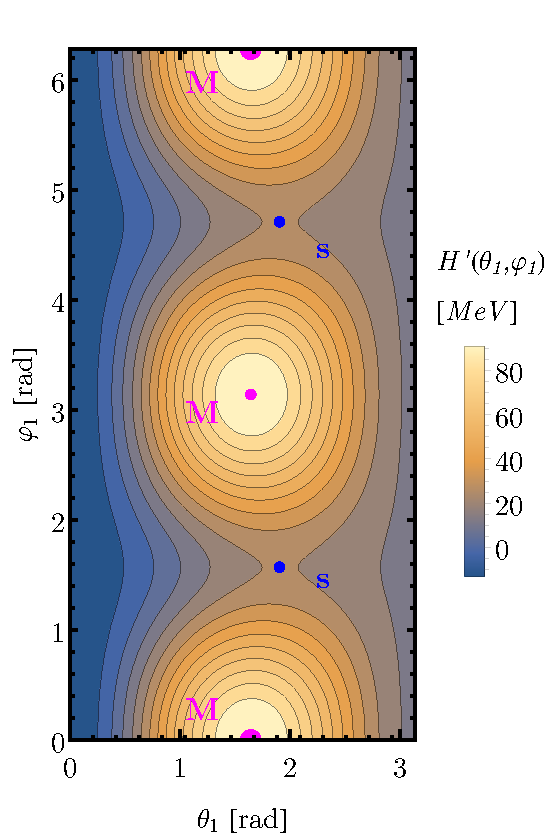
\includegraphics[scale=0.7]{Chapters/Figures/New-Boson-Classical-H-1axis-quantization.pdf}
        \caption{Contour plot for the energy $H'$ from Eq. \eqref{new-boson-h-prime-classical}, defined in terms of the polar coordinates. The calculations are done for $\mathcal{I}_1:\mathcal{I}_2:\mathcal{I}_3=80:10:50\ \hbar^2\text{MeV}^{-1}$ (i.e., the $1$-axis is the quantization axis). The single-particle angular momentum is $j=11/2$, the total angular momentum $I=19/2$, and $\theta=70^\circ$. The five stationary points are illustrated, namely three maxima (denoted by "M") and two saddle points (denoted by "s").}
        \label{new-boson-hprime-1axis-contour-plot}
    \end{center}
\end{figure}

The three situations A-B-C that were analyzed can be summarized with the following aspects:
\begin{itemize}
    \item there are six minima: A1, A2, B1, B2, and A3, C1 (when $u\in(-1,0)$)
    \item two maxima appear for the cases B3 and C2
    \item when $u\in(0,1)$, there are two saddle points: A3 and C1.
\end{itemize}

When the minimum points are considered, the total angular momentum is oriented along a principal axis (either the $1$- or $-1$-axis). However, for the maxima and saddle points, the angular momentum lies in a principal plane instead of being aligned along a preferred axis. The A3 and C1 cases result in a total a.m. that is oriented in the $(x_1,x_3$) plane. The stationary points are of minimum, maximum, or saddle character depending on the signs of the diagonal matrix elements of Hessian associated to $H'(\theta,\varphi)$. More precisely:
\begin{enumerate}
    \item \emph{minimum}: all the diagonal m.e. are positive
    \item \emph{saddle}: one m.e. is positive and one m.e. is negative
    \item \emph{maximum}: all the diagonal m.e. are negative
\end{enumerate}

If the Hessian is set to numerically vanish, then an equation is obtained for the parameters $u$ and $v\equiv v_0/I$ at which the critical points are degenerate:
\begin{align}
    (1-u)(1-v^2)(v^2-u^2)(v^2-u)=0\ .
    \label{new-boson-phase-diagram-parameter-equation}
\end{align}

Each factor from this equation will generate a curve within the $(u,v)$ plane (called a \emph{separatrix}). These separatrixes are bordering manifolds that define unique nuclear phases. This phase diagram is sketched in Fig. \ref{separatrix-diagram}. For the sake of completeness, the points corresponding to the values $(u,v)$ from the bases A-B-C are all represented on the same diagram, but with $v$ taken as an absolute value, to avoid negative ranges that are obtained when the $1$-axis is the quantization axis. Keep in mind that the different values for these parameters emerge from the change in the ordering of the three moments of inertia (recall Eq. \eqref{new-boson-hamiltonian-notations}).
\begin{figure}
    \centering
    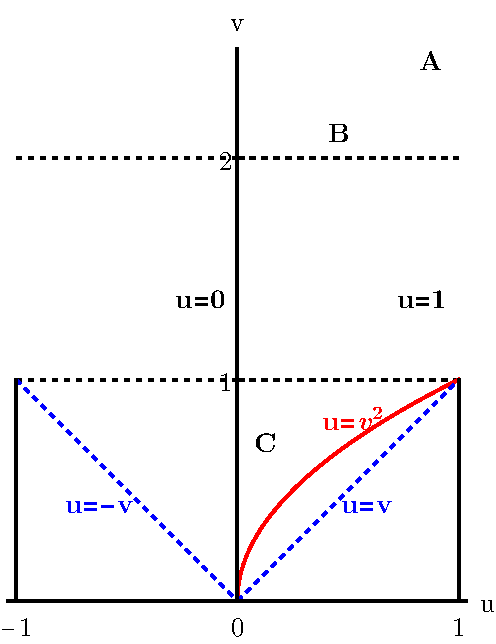
\includegraphics[scale=1]{Chapters/Figures/new-boson-separatrix-diagram.pdf}
    \caption{The phase diagram associated with the parametric formula given in Eq. \eqref{new-boson-phase-diagram-parameter-equation}. Each of the conditions that make the equation vanish is represented by a separatrix, such that different regions depict \emph{different nuclear phases}. The numerical values of $u$ and $v$ obtained from cases A-B-C are also represented within the plot.}
    \label{separatrix-diagram}
\end{figure}

\section{Electromagnetic Transitions}
\label{section-em-transitions-new-boson}

The next part of the team's work in Ref. \cite{raduta2020approach} was to obtain an analytical description for the electromagnetic operators, such that the boson model can be compared with real experimental data. Starting with the electric transitions, the wave function must be introduced. The wave function for a spin state $I$ must be \emph{the solution} of the Schrödinger equation for the total angular momentum $I$. Because i) the system is cranked around the $1$-axis and ii) the a.m. projection $I_1$ is equal to $-I$ in the minimum point, then the $K$ quantum number (i.e., the projection of $I$ on the $1$-axis in the intrinsic frame of reference) should also be $-I$. Thus, a solution to the Schrödinger equation could be employed:
\begin{align}
    \Psi_{IM}=\Phi_{I,-I}\ket{IM,-I}\ ,
\end{align}
where $\ket{IMK}$ are the Wigner-D functions, which were introduced and used in the previous chapters (see Eq. \eqref{IMK-wigner-functions}).

For the \emph{quadrupole transition operator}, the following expression was used (slightly modified when compared to Eq. \eqref{electric-quadrupole-operator-lab}):
\begin{align}
    \mathcal{M}\left(E_2;\mu\right)=\sqrt{\frac{5}{16\pi}}\mathrm{e}\left(Q_{2-2}\mathcal{D}_{\mu -2}^2+Q_{20}\mathcal{D}_{\mu 0}^2+Q_{22}\mathcal{D}_{\mu 2}^2\right)\ ,
\end{align}
with $Q_{20}$ and $Q_{2\pm2}$ denoting the $K=\{-2,0,2\}$ components of the quadrupole transition operator. From the expressions of the wave function given in Eq. \eqref{schrodinger-equation-elliptic}, it is clear that it will depend on the conjugate variables $q$ and $d/dg$. For this reason, the quadrupole components need to be expressed as functions of these variables. If the components are firstly written in terms of the angular momentum, one has:
\begin{align}
    Q_{20}=\left(-\frac{1}{4}\sqrt{\frac{2}{3}}\left(\hat{I}_+\hat{I}_-+\hat{I}_-\hat{I}_+\right)+\sqrt{\frac{2}{3}}\hat{I}_1^2\right)\bar{Q}_0\ ,\ Q_{2\pm2}=\frac{1}{2}\hat{I}_\pm^2\bar{Q}_2\ .
\end{align}

The factors $\bar{Q}_0$ and $\bar{Q}_2$ are the \emph{intrinsic quadrupole components}. Then, by using the Bargmann representation of the a.m. components, around the minimum point $Q_{20}$ and $Q_{2\pm2}$ become \cite{raduta2020new}:
\begin{align}
    Q_{20}&=\frac{1}{\sqrt{6}}\left[3\bar{q}^2\frac{d^2}{d\bar{q}^2}-3(2I-1)\bar{q}\frac{d}{d\bar{q}}+I(2I-1)-I(I-1)(1+k^2)\bar{q}^2\right]\bar{Q}_0\ ,\nonumber\\
    Q_{2\pm2}&=\frac{1}{k'^2}\left\{\left[(1+k^2)\bar{q}^2-2\right]\frac{d^2}{d\bar{q}^2}-(2I-1)(1+k^2)\bar{q}\frac{d}{d\bar{q}}\right\}\bar{Q}_2\times \nonumber\\
    &\times\frac{1}{k'^2}\left\{I\left[(I+1)(1+k^2)+k^2(k^2+3)\right]\bar{q}^2-I(1+k^2)\right\}\bar{Q}_2\ .
\end{align}

To calculate the matrix elements of the transition operator, the overlap factors for the interband and intraband transitions need to be determined. As per the calculations of Ref. \cite{raduta2020new}, it was shown that both $\bra{\Phi_{I,-I}}\ket{\Phi_{I-1,-I+1}}$ and $\bra{\Phi_{I,-I}}\ket{\Phi_{I-2,-I+2}}$ are very close to unity, such that they can be fixed to $1$. The reduced transition probabilities can be evaluated using the following formula:
\begin{align}
    B(E2;I\to I')=\left|\bra{\psi_I}|\mathcal{M}(E2)|\ket{\Psi_{I'}}\right|^2\ .
    \label{reduced-electric-quadrupole-new-boson}
\end{align}

The intrinsic quadrupole moments $\bar{Q}_2$ and $\bar{Q}_0$ are taken as \emph{free parameters} within this approach, and the matrix elements for $\bra{\Psi_I}|\mathcal{M}(E2)|\ket{\Psi_{I-2}}$ (intraband) and $\bra{\Psi_I}|\mathcal{M}(E2)|\ket{\Psi_{I-1}}$ (interband) are given analytically in Eqs. (6.5) and (6.6) from Ref. \cite{raduta2020new}.

The \emph{magnetic dipole transition} operator is defined as \cite{raduta2020new}:
\begin{align}
    \mathcal{M}\left(M1;\mu\right)=\frac{3}{4\pi}\mu_N\sum_{\nu}\left(g_R\hat{R}_\nu+g_j\hat{j}_\nu\right)\mathcal{D}_{\mu\nu}^1\equiv M_{1\mu}^\text{coll}+M_{1\mu}^\text{sp}\ ,
\end{align}
where the terms $R_\nu$ and $j_\nu$ are the spherical components of the core and the odd single-particle. The gyromagnetic factors of the core and the particle are denoted by $g_R$ and $g_j$, respectively. The matrix elements of the collective and single-particle transition operators $M_{1\mu}^\text{coll}$ and $M_{1\mu}^\text{sp}$ are provided in the set of Eqs. (6.10) - (6.12) from Ref. \cite{raduta2020new}. Therein, the values for the gyromagnetic factors are provided as well. These are used to get the analytical expression of the reduced transition probability for the magnetic dipole:
\begin{align}
    B(M1;I\to I')=\left|\bra{\Psi_{I}}|\mathcal{M}(M1)|\ket{\Psi_{I'}}\right|^2\ .
    \label{reduced-magnetic-dipole-new-boson}
\end{align}

\section{Numerical Results}
\label{numerical-results-new-boson}

The entire formalism developed through Ref. \cite{raduta2020new} was tested numerically for the odd-$A$ nucleus $^{135}$Pr. This odd-mass nucleus was chosen because experimental evidence point out its wobbling character \cite{matta2017transverse} (and later erratum in Ref. \cite{matta2021erratum}), although there are some ongoing debates about whether the experimental measurements are valid or not \cite{guo2021comment}. For this isotope, there are three confirmed wobbling bands, here denoted by B1 (band one), B2 (band two), and B3 (band three). Sensharma et. al. \cite{sensharma2019two} consider in their study for this nucleus that B1 is the yrast, B2 is the one-phonon, and finally that B3 is the two-phonon wobbling band. By contrast, a previous work by Matta et. al. \cite{matta2017transverse} only identified one such excited wobbling band.

The formalism assumes that the problem is described by a Hamiltonian such as the one from Eq. \eqref{rotor-hamiltonian-new-boson}, which is associated with the even-even core surrounded by an odd nucleon: the odd $h_{11/2}$ proton. The core is considered to have a set of moments of inertia $\mathcal{I}_k$ ($k=1,2,3$) that are \emph{free parameters}. Moreover, the proton is \emph{rigidly coupled} to the core and placed in the $(1,2)$-plane, with the tilting angle $\theta$. As a result, the model only considers four free parameters, i.e., three moments of inertia and the single-particle tilt:
\begin{align}
    \mathcal{P}_\text{fit}=\left[\mathcal{I}_1\ ,\ \mathcal{I}_2\ ,\ \mathcal{I}_3\ ,\ \theta\right]\ .
\end{align}
These values are determined via a fitting procedure for the three wobbling bands in $^{135}$Pr. The adopted fitting procedure is quite similar to the one that the team developed for $\mathbf{W_1}$ and $\mathbf{W_2}$, but any key difference will be pointed out in the following sections.

\subsection{Excitation Energies}

The bands B1 and B2 are signature partner bands, having an opposite signature quantum number ($+1/2$ for the favored and $-1/2$ for the unfavored). Due to this reason, the wobbling phonon numbers are $n_{B1}=n_{B2}=0$ for the first two bands and $n_{B3}=1$ for the third, meaning that B3 is a one-phonon excitation (band B3 is a \emph{one-phonon excitation} of B2). This is similar to the condition employed in the $\mathbf{W_1}$ approach, where one studied the electromagnetic properties of several Lu isotopes. Since the \emph{excitation energies} are obtained by subtracting the band-head $E_{I_b}$ value ($I_b$ signifies the spin of the true ground state of the yrast band B1), one must consider the analytical expressions \cite{raduta2020new}:
\begin{align}
    E_I^\text{exc;B1}&=A_1I^2+(2I+1)A_1j_1-IA_2j_2+\frac{1}{2}\omega_I-E_{11/2}\ ,\nonumber\\
    I&=R+j\ ,R=0,2,4,\dots\ \in\text{B1}\ ,\nonumber\\
    E_I^\text{exc;B2}&=A_1I^2+(2I+1)A_1j_1-IA_2j_2+\frac{1}{2}\omega_I-E_{11/2}\ ,\nonumber\\
    I&=R+j\ ,R=1,3,5,\dots\ \in\text{B2}\ ,\nonumber\\
    E_I^\text{exc;B3}&=A_1I^2+(2I+1)A_1j_1-IA_2j_2+\frac{3}{2}\omega_I-E_{11/2}\ ,\nonumber\\
    I&=R+j\ ,R=1,3,5,\dots\ \in\text{B3}\ ,
    \label{excitation-energies-new-boson}
\end{align}
where it can be seen that the analytical formulas for the first two bands are identical, but the angular momenta will differ by one unit. The band B3 being a one-phonon excitation, a state $I+1$ is obtained by exciting with one-wobbling quanta the $I$ state from B2. The \emph{wobbling frequency} $\omega_I$ is an angular-momentum dependent function given as \cite{raduta2020new}:
\begin{align}
    \omega_I^2=&\left[(2I+1)\left(A_2-A_1-\frac{A_2j_2}{I}\right)+2A_1j_1\right]\left[(2I+1)(A_3-A_1)+2A_1j_1\right]-\nonumber\\
    &-(A_3-A_1)\left(A_2-A_1-\frac{A_2j_2}{I}\right)\ .
    \label{wobbling-frequency-new-boson}
\end{align}

In order to understand Eq. \eqref{excitation-energies-new-boson}, one might recall the diagram from Fig. \ref{fitting-workflow-fig}, which shows how the excitation energies can be regarded. The parameters $\mathcal{P}_\text{fit}$ obtained by fitting the experimental energies of $^{!35}$Pr with Eq. \eqref{excitation-energies-new-boson} are provided in Table \ref{new-boson-fitting-parameters}. It should be mentioned that several conditions were restricted when searching for $\mathcal{P}_\text{fit}$ (i.e., some sort of \emph{validity conditions}):
\begin{itemize}
    \item The factor $A$ must be greater than zero (recall Eq. \eqref{new-boson-hamiltonian-notations})
    \item The factor $u$ from the same equation must be $u\in(0,1)$
    \item The wobbling frequency $\omega_I$ as well as the one obtained by expanding $H'$ around the local minimum (that is $\omega'_I$ from Eq. \eqref{wobbling-frequency-new-boson-prime}) must be real functions of $\theta$ and $\theta+\pi$
    \item The elliptic potential from Eq. \eqref{elliptic-potential-formula} must be a real function for $\theta$ and $\theta+\pi$.
\end{itemize}
\begin{table}
    \centering
    \caption{The four free parameters obtained by fitting the experimental energies of $^{135}$Pr (taken from Ref. \cite{matta2017transverse}) using the set of energies from Eq. \eqref{excitation-energies-new-boson}. For the moments of inertia, the unit is $\hbar^2\text{MeV}^{-1}$.}
    \resizebox{0.8\textwidth}{!}{%
    \begin{tabular}{cccccc}
    \hline
    $\mathcal{I}_1$ & $\mathcal{I}_2$ & $\mathcal{I}_3$ & $\theta\ \left[\text{degrees}\right]$ & N.o. states & $\text{RMS}\ \left[\text{MeV}\right]$\ \\ \hline \hline
    91 & 9 & 51 & $-119$ & 20 & 0.174 \\ \hline
    \end{tabular}%
    }
    \label{new-boson-fitting-parameters}
\end{table}

With these criteria in check, the fitting procedure was performed and calculations gave an RMS of about $0.170\ \text{MeV}$. Comparing this work with other models from the literature, such as Ref. \cite{chen2016wobbling} ($\approx0.160\ \text{MeV}$) and Ref. \cite{budaca2018tilted} ($\approx0.150\ \text{MeV}$) it can be concluded that a semi-classical analysis of the boson description for odd-mass wobbling nuclei is quite realistic. The excitation energies for all three bands are graphically represented as level schemes in Figs. \ref{135pr-new-boson-band1} - \ref{135pr-new-boson-band23}. From these figures, a few points are worth mentioning. For example, it can be seen that for B1 the model gives slightly larger excitation energies across the spectrum, especially for the states close to the band-head and the most excited states. For B2, the slightly larger theoretical energies are obtained for the low-spin region, while the end of the spectrum is a bit underestimated. Interestingly, the one-phonon wobbling band seems to be described very accurately by the model, without any noticeable differences. 
\begin{figure}[t] % temporary force to the top - prevents intersection with the previous itemize/table
    \centering
    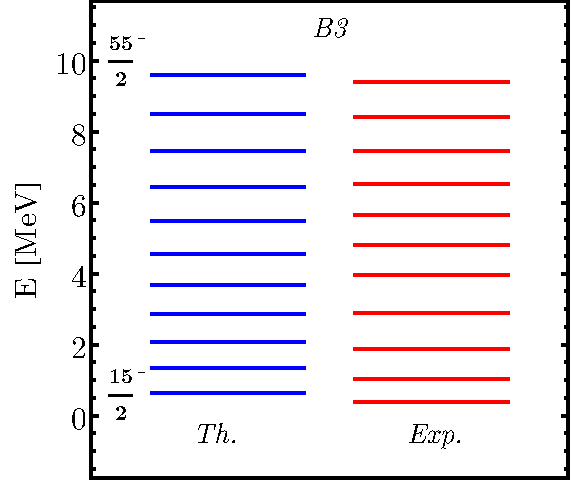
\includegraphics[width=0.49\textwidth]{Chapters/Figures/135Pr-New-Boson-Band1-Energies.pdf}
    \caption{The excitation energies $E_I^\text{exc;B1}$ in $^{135}$Pr (Eq. \eqref{excitation-energies-new-boson}), calculated with the parameter set $\mathcal{P}_\text{fit}$. The experimental data are taken from Ref. \cite{sensharma2019two}.}
    \label{135pr-new-boson-band1}
\end{figure}
\begin{figure}[b] % temporary force to the bottom - prevents intersection with the previous figure
    \centering
    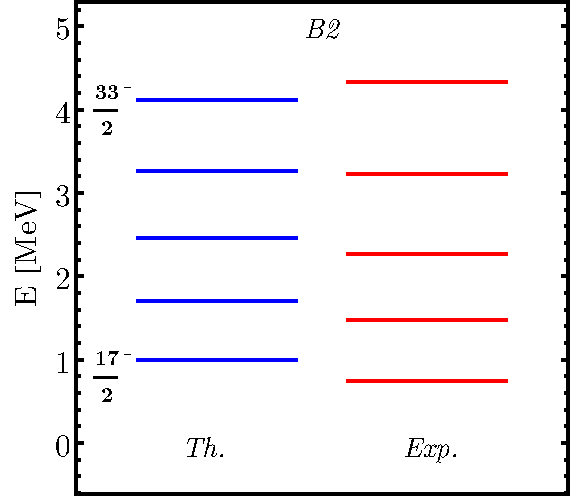
\includegraphics[width=0.49\textwidth]{Chapters/Figures/135Pr-New-Boson-Band2-Energies.pdf}
    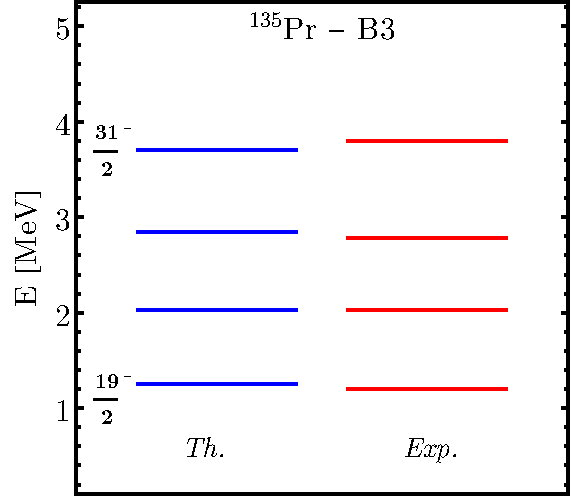
\includegraphics[width=0.49\textwidth]{Chapters/Figures/135Pr-New-Boson-Band3-Energies.pdf}
    \caption{The excitation energies $E_I^\text{exc;B2}$ (\textbf{left}) and $E_I^\text{exc;B3}$ (\textbf{right}) in $^{135}$Pr (Eq. \eqref{excitation-energies-new-boson}), calculated with the parameter set $\mathcal{P}_\text{fit}$. The experimental data are taken from Ref. \cite{sensharma2019two}.}
    \label{135pr-new-boson-band23}
\end{figure}

Taking a closer look at the numerical values from Table \ref{new-boson-fitting-parameters}, it can be seen that the fit predicted the MOI order to be of the type $\mathcal{I}_1>\mathcal{I}_3>\mathcal{I}_2$. With these values, one can graphically represent the elliptic potentials for $V(\theta)$ and $V(\theta+\pi)$, as provided by Eq. \eqref{elliptic-potential-formula}. The results are shown in Fig. \ref{elliptic-potential-theta} for three values of angular momentum $I$ and the two angles.
\begin{figure}[b] % temporary force to the bottom
    \centering
    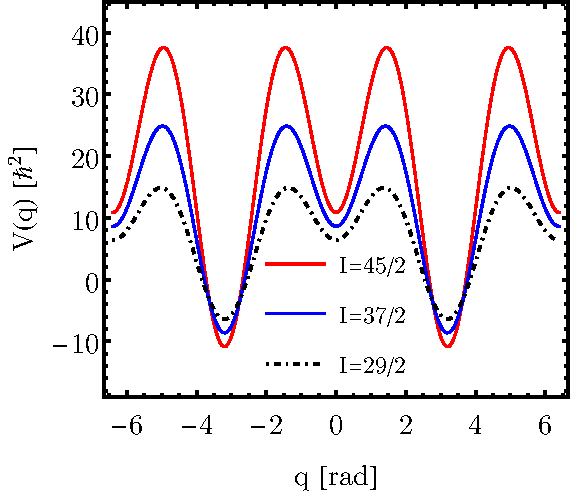
\includegraphics[width=0.49\textwidth]{Chapters/Figures/potential-fit-theta.pdf}
    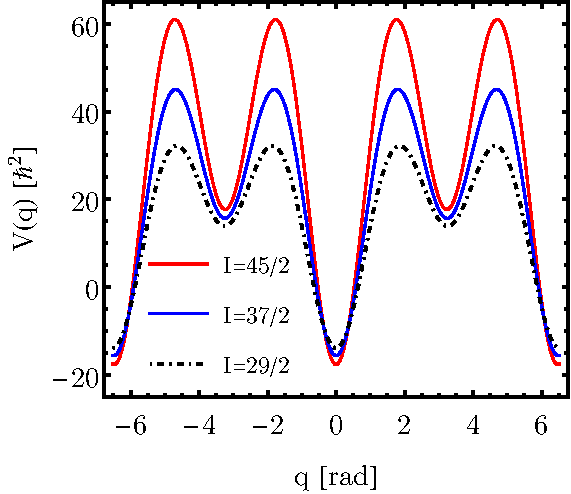
\includegraphics[width=0.49\textwidth]{Chapters/Figures/potential-fit-theta-pi.pdf}
    \caption{The elliptic potential from Eq. \eqref{elliptic-potential-formula} as function of the coordinate $q$. The expression of $V(q)$ is evaluated for the inertia factors from Table \ref{new-boson-fitting-parameters} with $\theta=-119^\circ$ (\textbf{left}) and $\theta=61^\circ$ (\textbf{right}).}
    \label{elliptic-potential-theta}
\end{figure}

Looking at the two potentials associated with $^{135}$Pr from Fig. \ref{elliptic-potential-theta}, several features can be observed. Firstly, the deepest minimum for $\theta$ is located at $2K$, while for $\theta+\pi$ is at $q=0$ (recall that $K$ is the period of the elliptic functions used to express $V(q)$). This is remarkable since it contrasts the initial consideration of $\mathcal{I}_2$ as being the maximal MOI, which should have the global minima located at $q=0$. One reason might be the coupling between the even-even core and the odd nucleon, as their interaction can affect both the MOI's ordering and the position of the deepest minimum for the triaxial potential. It is a unique highlight of the boson description where such an effect is identified. Because the global minimum for $\theta+\pi$ stays at $q=0$, one can assert that by drastically switching the orientation angle between the odd-particle and the core, a \emph{phase transition occurs}, affecting the MOI from $\mathcal{I}_1=\mathcal{I}_\text{max}$ to $\mathcal{I}_2=\mathcal{I}_\text{max}$.

Aiming at the initial assumption of $\mathcal{I}_2$ as the largest NOI, a second fitting procedure was also developed. The fit consisted of equating the excitation energies for the first two states in B1 and the second state from B2. A parameter set that suits the MOI order was obtained for $\theta=140^\circ$: $\mathcal{P}_\text{fit}=\left[13,101,53,140^\circ\right]$. However, this parameter set does not improve the quality of the initial fit, keeping the deviations from the experimental values along the same magnitude. For this set of parameters, the elliptic triaxial potential has the deepest minimum at $q=0$, which is consistent with the $\mathcal{I}_2>\mathcal{I}_{1,3}$. This solution is not valid because it violates the positivity condition for the factor $A$ from Eq. \eqref{new-boson-hamiltonian-notations}.

Since the potential when $\theta=-114^\circ$ has the global minimum in $q=2K$, it is worth adjusting the fitting model and using the wobbling frequency $\omega'$ from Eq. \eqref{wobbling-frequency-new-boson-prime} for the excitation energies. The expression of $\omega'$ was obtained by expanding $V(q)$ up to second order in the local minima $q=\pm 2K$, making it perfectly suitable for the calculus of the excitation energies from in Eq. \eqref{excitation-energies-new-boson}. Indeed, repeating the fitting procedure the results are $\mathcal{P}_\text{fit}=\left[89,12,48,-71^\circ\right]$. This also provides an RMS that is similar to the initial one. It is somewhat expected that the change in the wobbling frequency $\omega\rightarrow\omega'$ would lead to similar excitation energies, as they differ by a constant amount, independent of $I$ \cite{raduta2020new}. For the sake of completeness, the elliptic potential $V(q)$ is graphically represented for the set of MOI, $\theta$, and $\theta+\pi$ given by the alternative fitting procedures in Figs. \ref{elliptic-potential-theta2} - \ref{elliptic-potential-theta3}.
\begin{figure}
    \centering
    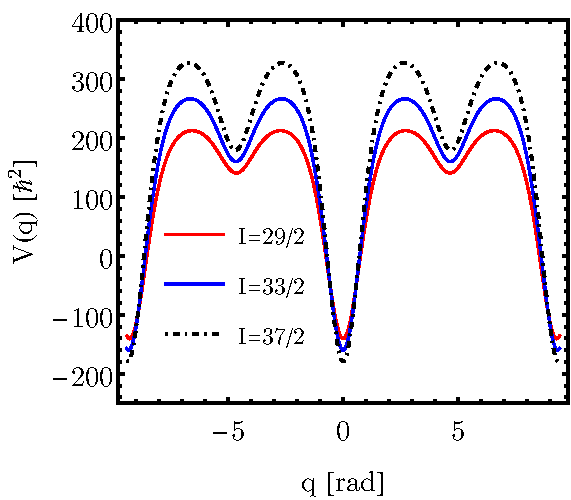
\includegraphics[width=0.49\textwidth]{Chapters/Figures/potential-fit2-theta.pdf}
    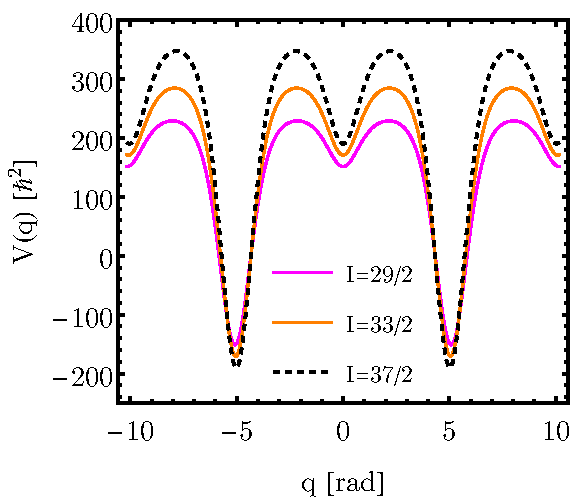
\includegraphics[width=0.49\textwidth]{Chapters/Figures/potential-fit2-theta-pi.pdf}
    \caption{The triaxial potential from Eq. \eqref{elliptic-potential-formula} associated to $^{135}$Pr, evaluated for the case of maximal MOI along $2$-axis. The three MOI are $\mathcal{I}_1:\mathcal{I}_2:\mathcal{I}_3\approx13:101:53\ \hbar^2\text{MeV}^{-1}$, $\theta=140^\circ$ (\textbf{left}), and $\theta=320^\circ$ (\textbf{right}).}
    \label{elliptic-potential-theta2}
\end{figure}
\begin{figure}
    \centering
    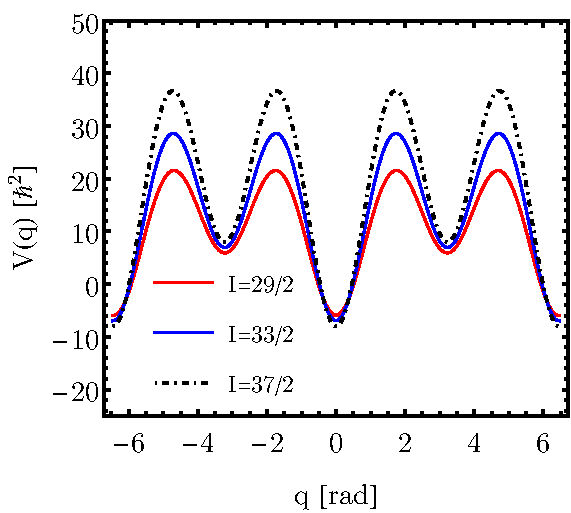
\includegraphics[width=0.49\textwidth]{Chapters/Figures/potential-fit3-theta.pdf}
    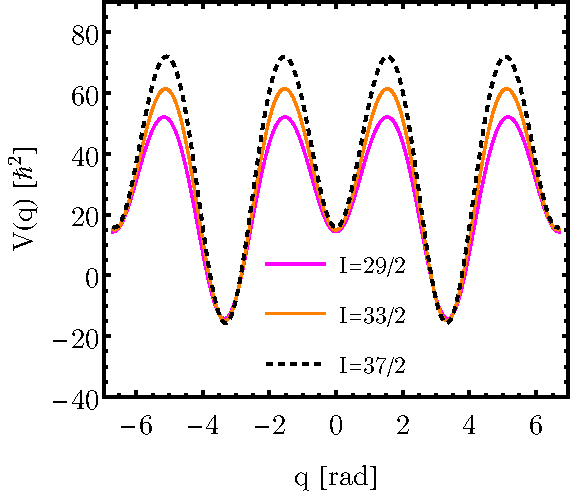
\includegraphics[width=0.49\textwidth]{Chapters/Figures/potential-fit3-theta-pi.pdf}
    \caption{The triaxial potential from Eq. \eqref{elliptic-potential-formula} associated to $^{135}$Pr, evaluated using $\omega'$ instead of $\omega$ (see Eq. \eqref{wobbling-frequency-new-boson-prime}). The MOI are: $\mathcal{I}_1:\mathcal{I}_2:\mathcal{I}_3\approx89:12:48\ \hbar^2\text{MeV}^{-1}$, $\theta=-71^\circ$ (\textbf{left}), and $\theta=109^\circ$ (\textbf{right}).}
    \label{elliptic-potential-theta3}
\end{figure}

Taking a look at all three sets of potentials from Figs. \ref{elliptic-potential-theta} - \ref{elliptic-potential-theta3}, it can be seen that except for the case of $\mathcal{I}_2=\mathcal{I}_\text{max}$, the $V(q)$ ranges are quite close to each other. The very large values for $V(q)$ from Fig. \ref{elliptic-potential-theta2} show that the transverse wobbling for $^{135}$Pr is unstable. Notice the alternating character of the deepest minima for the angle $\theta$ (i.e., between the plots for $\theta$ and $\theta+\pi$). The very sharp minimum points also indicate that the core + particle interaction stabilizes near $q=0,2K,\dots$. 

The wobbling frequency for $^{135}$Pr can be easily determined by using the moments of inertia and the angle $\theta$ in the analytical expressions from Eq. \eqref{omega-frequency-deepest-minima} for $\omega$ and Eq. \eqref{wobbling-frequency-new-boson-prime} for $\omega'$, respectively. A set of graphical representations are made in Figs. \ref{wobbling-frequencies-135pr-fit1} - \ref{wobbling-frequencies-135pr-fit3} where each plot is generated using the numerical values from Table \ref{new-boson-fitting-parameters} (for the first set of plots), the fit when $\mathcal{I}_2=\mathcal{I}_\text{max}$ (second set of plots), and lastly, the fit when the excitation energies are evaluated with $\omega'$ (third set of plots).
\begin{figure}
    \centering
    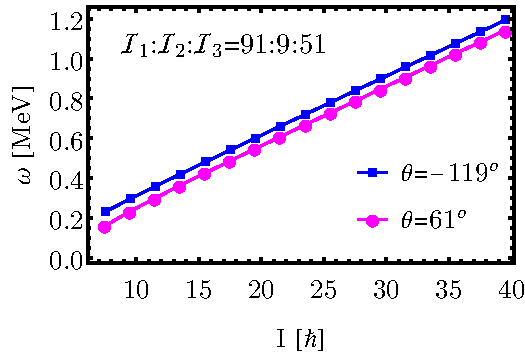
\includegraphics[width=0.49\textwidth]{Chapters/Figures/omega-fit-1.pdf}
    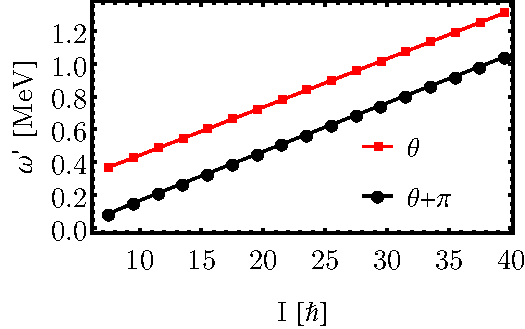
\includegraphics[width=0.49\textwidth]{Chapters/Figures/omega-prime-fit-1.pdf}
    \caption{The wobbling frequency as function of angular momentum for $^{135}$Pr, according to Eq. \eqref{omega-frequency-deepest-minima} (\textbf{left}) and Eq. \eqref{wobbling-frequency-new-boson-prime} (\textbf{right}). The calculations are done for the parameters provided in Table \ref{new-boson-fitting-parameters}. The value $\langle\delta\rangle$ represents the average spacing between the two frequencies (see text for more details).}
    \label{wobbling-frequencies-135pr-fit1}
\end{figure}
\begin{figure}
    \centering
    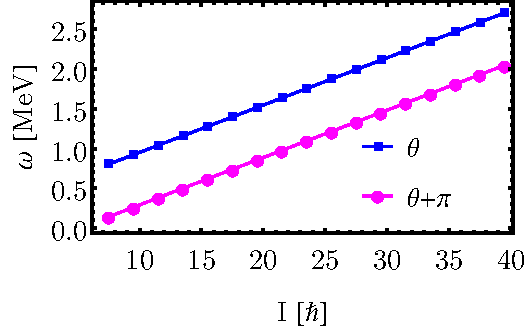
\includegraphics[width=0.49\textwidth]{Chapters/Figures/omega-fit-2.pdf}
    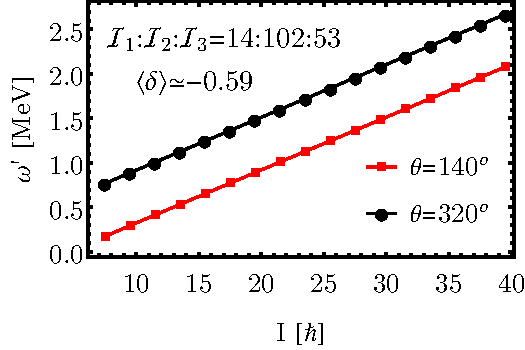
\includegraphics[width=0.49\textwidth]{Chapters/Figures/omega-prime-fit-2.pdf}
    \caption{The wobbling frequency as function of angular momentum for $^{135}$Pr, according to Eq. \eqref{omega-frequency-deepest-minima} (\textbf{left}) and Eq. \eqref{wobbling-frequency-new-boson-prime} (\textbf{right}). The calculations are done for the parameters obtained by fitting Eq. \eqref{excitation-energies-new-boson} such that $\mathcal{I}_2=\mathcal{I}_\text{max}$. The value $\langle\delta\rangle$ represents the average spacing between the two frequencies (see text for more details).}
    \label{wobbling-frequencies-135pr-fit2}
\end{figure}
\begin{figure}
    \centering
    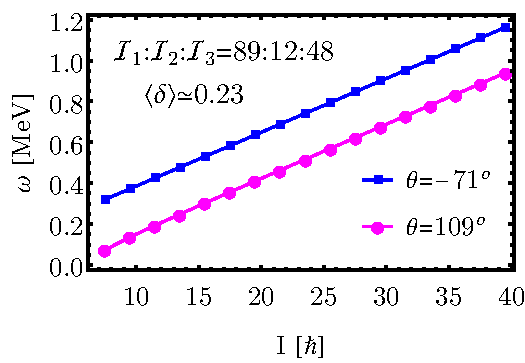
\includegraphics[width=0.49\textwidth]{Chapters/Figures/omega-fit-3.pdf}
    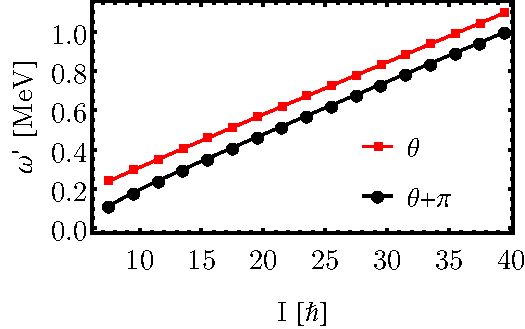
\includegraphics[width=0.49\textwidth]{Chapters/Figures/omega-prime-fit-3.pdf}
    \caption{The wobbling frequency as function of angular momentum for $^{135}$Pr, according to Eq. \eqref{omega-frequency-deepest-minima} (\textbf{left}) and Eq. \eqref{wobbling-frequency-new-boson-prime} (\textbf{right}). Results were achieved with the parameters given by a fit of Eq. \eqref{excitation-energies-new-boson} using $\omega'$ in its analytical expression. The value $\langle\delta\rangle$ represents the average spacing between the two frequencies (see text for more details).}
    \label{wobbling-frequencies-135pr-fit3}
\end{figure}

Note the linear behavior of the phonon energy w.r.t. angular momentum. Moreover, the energy for $\omega$ lies higher in magnitude than its $\theta+\pi$ partner, except for the case of $2$-axis quantization (that is Fig. \ref{wobbling-frequencies-135pr-fit2}), where it can be seen that $\omega'(\theta+\pi)$ is larger. In terms of the differences between the frequency evaluated for $\theta$ and $\theta+\pi$, they are quite constant across the entire spin range for all figures, with the smallest difference achieved for $\omega$ from Fig. \ref{wobbling-frequencies-135pr-fit1}. If the difference between $\omega(\theta)$ and $\omega(\theta+\pi)$ for a given angular momentum $I$ is denoted by $\delta(\omega_I)$:
\begin{align}
\delta(\omega_I)=\omega(\theta)-\omega(\theta+\pi)\ ,    
\end{align}
then one can compute the average $\langle\delta\rangle$ across each of the three sets of figures. The same can be done for $\delta(\omega'_I)$, and these numbers are shown on all six plots.

\subsection{On the Chiral Character of the Wobbling Motion}
\label{new-boson-chiral-character}

As discussed in the chapter dedicated to the signatures of triaxial nuclei (recall Section \ref{subsection-chiral-motion}), the \emph{chirality} corresponds to a transformation that brings a right-handed system into a left-handed one. The change of the sign for the a.m. defines the chiral transformation itself. Thus, the invariance to a chiral transformation is given by the conservation of the rotational energy when the rotational axis is changed. Referring back to the initial Hamiltonian from Eq. \eqref{rotor-hamiltonian-new-boson}, this consists of a sum of two terms, one that is symmetric to a chiral transformation and one that is antisymmetric:
\begin{align}
    \hat{H}_\text{rot}=\hat{H}_\text{symm}+\hat{H}_\text{asymm}\ .
\end{align}

If $\ket{\Psi}$ is an eigenstate for the symmetric Hamiltonian and $\hat{C}$ defines a chiral transformation, then $\hat{C}\ket{\Psi}$ is also an eigenstate for $\hat{H}_\text{symm}$, and it corresponds to the same eigenvalue. From the equality:
\begin{align}
    \hat{C}\ket{\Psi}=\ket{\Psi}\ ,
\end{align}
it results that the state has a chirality equal to one. On the other hand, if $\ket{\Phi}$ is an eigenstate for the asymmetric term with an eigenvalue $E$, then $\hat{C}\ket{\Phi}$ is also an eigenstate for $\hat{H}_\text{asymm}$, but it will correspond to the energy $-E$. The eigenvalues of $\hat{H}_\text{asymm}$ split into two groups; each being the mirror image of the other. Such a property is said to be \emph{of chiral type}. The chirality for the eigenstates of $\hat{H}_\text{asymm}$ is negative (i.e., $-1$), since $\hat{C}\ket{\Phi}=-\ket{\Phi}$.

Based on the description of the chirality for $\hat{H}_\text{symm}$ and $\hat{H}_\text{asymm}$, the eigenstates for the total Hamiltonian $\hat{H}_\text{rot}$ are mixtures of the two types of chirality: positive and negative. Within the calculations performed in this chapter for $^{135}$Pr, the change $\mathbf{I}\rightarrow\mathbf{-I}$ is obtained by changing the orientation angle of the single-particle from $\theta$ to $\theta+\pi$. All the calculations that were graphically represented for $V(q)$ and $\omega$ in the previous subsection were made for the orientation of the nucleon that emerged from the fitting procedure and the \emph{chiral transformed} one. If the potential evaluated for $\theta$ is $V$, then the chiral potential for $\theta+\pi$ is indeed $\hat{C}V\hat{C}^{-1}$. From the potential energy represented throughout Figs. \ref{elliptic-potential-theta} - \ref{elliptic-potential-theta3}, one can extract the \emph{symmetric} and \emph{asymmetric} parts:
\begin{align}
    V_\text{symm}&=\frac{1}{2}\left(V_\theta+V_{\theta+\pi}\right)\ , \nonumber \\
    V_\text{asymm}&=\frac{1}{2}\left(V_\theta-V_{\theta+\pi}\right)\ .
    \label{chiral-potentials-symmetric-asymmetric}
\end{align}

The symmetric and asymmetric potentials are represented as a function of the coordinate $q$ in Fig. \ref{chiral-potentials-plot}, for the moments of inertia and the single-particle orientation angle provided by fitting the excitation energies of Eq. \eqref{excitation-energies-new-boson}. For keeping a concise representation, only $I=45/2$ was considered. Note the oscillatory character of $V_\text{symm}$ that is more pronounced, with very deep minima and maxima across the $q$ range. The asymmetric potential is almost flat when $q\approx2K$.

The elliptic triaxial potential $V(q)$ expressed in Eq. \eqref{elliptic-potential-formula} is a function that depends explicitly on the elliptic modulus $k$. Moreover, the modulus was defined in terms of the factor $u=(A_3-A_1)/A$ (recall Eq. \eqref{new-boson-hamiltonian-notations}). From that formula, it is obvious that $k$ will change when $\theta$ changes, through the re-adjustment of the single-particle a.m. components $j_1$ and $j_2$. As a result, the period $K$ (which gives the location of critical points) will also depend on the orientation angle $\theta$. When comparing $V_\text{symm}$ and $V_\text{asymm}$ for a shared set of coordinates $q$, an offset $\Delta K=\left|K_\theta-K_{\theta+\pi}\right|$ is required to compensate for the difference in their periods.
\begin{figure}
    \centering
    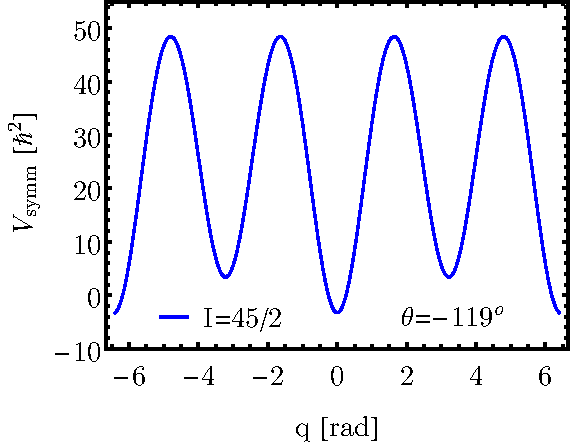
\includegraphics[width=0.49\textwidth]{Chapters/Figures/symmetric-potential-135Pr.pdf}
    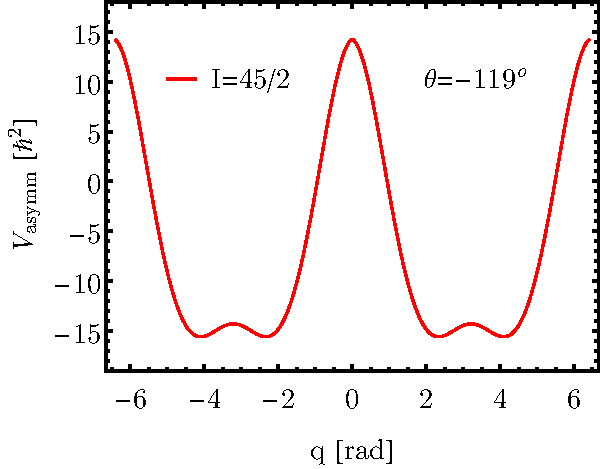
\includegraphics[width=0.49\textwidth]{Chapters/Figures/asymmetric-potential-135Pr.pdf}
    \caption{The symmetric \textbf{left} and asymmetric \textbf{right} potentials from Eq. \eqref{chiral-potentials-symmetric-asymmetric} associated to $^{135}$Pr. The numerical evaluation is done with the fitting parameters from Table \ref{new-boson-fitting-parameters}.}
    \label{chiral-potentials-plot}
\end{figure}

The excitation energies from Eq. \eqref{excitation-energies-new-boson} can also be \emph{decomposed} into symmetric and asymmetric terms. For the yrast states (i.e., the band B1) the \emph{chiral pair} of excitation energies are defined as \cite{raduta2020new}:
\begin{align}
    \centering
    E_I^\text{exc;B1}(\text{symm})&=A_1I^2+\frac{1}{2}\left[\omega_I(\theta)+\omega_I(\theta+\pi)\right]\ ,\nonumber\\
    E_I^\text{exc;B1}(\text{asymm})&=(2I+1)A_1j_1-IA_2j_2+\frac{1}{2}\left[\omega_I(\theta)-\omega_I(\theta+\pi)\right]\ ,
    \label{excitation-energies-new-boson-symm-asymm}
\end{align}
where it can be seen that the wobbling frequency $\omega(\theta)$ and its \emph{chiral partner} $\omega(\theta+\pi)$ appear. For the set of MOI provided in Table \ref{new-boson-fitting-parameters} and $\theta=-119^\circ$, the symmetric and asymmetric excitation energies for B1 are numerically evaluated and plotted against the total spin $I$ in Figs. \ref{chiral-excitation-energies-135Pr}.
\begin{figure}
    \centering
    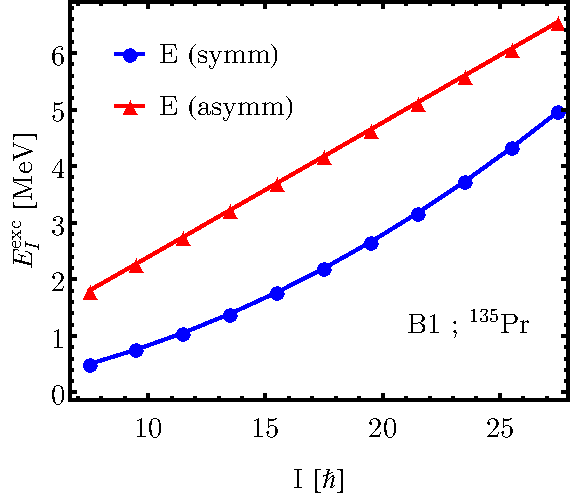
\includegraphics[scale=0.8]{Chapters/Figures/chiral-excitation-energies-135Pr.pdf}
    \caption{The symmetric and asymmetric excitation energies from Eq. \eqref{excitation-energies-new-boson-symm-asymm} for $^{135}$Pr, evaluated for the parameters given in Table \ref{new-boson-fitting-parameters}. The lines connecting the dots are just to guide the eye.}
    \label{chiral-excitation-energies-135Pr}
\end{figure}

The two sets of excitation energies $E(\text{symm})$ and $E(\text{asymm})$ correspond to two bands of opposite chirality. Indeed, the symmetric values correspond to a symmetric Hamiltonian and chirality $+1$, while the asymmetric values have negative chirality $-1$ and belong to an asymmetric Hamiltonian. Looking at Fig. \ref{chiral-excitation-energies-135Pr}, it can be seen that both bands are relatively close to each other, and they almost have similar behavior for the total angular momentum. Nevertheless, the quadratic increase of $E(\text{symm})$ is noticeable. The rather constant energy spacing between the two bands is a feature specific to chiral bands \cite{raduta2020new} (see the chiral bands from Figs. \ref{chiral-bands-1} - \ref{chiral-bands-2}). The fact that the initial Hamiltonian contains a linear term is another feature of the chiral motion, which means that the wobbling and chiral properties seem to be somewhat connected for $^{135}$Pr. This is the first time both phenomena are studied on the same family of bands, and the only property that holds against a decisive unified character of wobbling and chiral bands in $^{135}$Pr would be the rotational axis (that is, for a chiral nucleus, the rotational axis lies outside any of the principal planes - recall Fig. \ref{chiral-geometry}). More experimental data on this isotope would help to conclude whether these two bands are of a chiral type or not. 
\subsection{Electromagnetic Transitions}

The E2 and M1 reduced transition probabilities are calculated according to Eq. \eqref{reduced-electric-quadrupole-new-boson} and Eq. \eqref{reduced-magnetic-dipole-new-boson}, respectively. The initial and final wave functions are determined from the calculus of energies, connecting in this way the electromagnetic transitions to the model Hamiltonian. As already mentioned, the numerical values for these quantities require two adjustable parameters: $\bar{Q}_0$ and $\bar{Q}_2$. The parameters used in this work are \cite{raduta2020new}:
%TO-DO add the fitting method description
\begin{align}
    \bar{Q}_0=-30.02\ \mathrm{e}\cdot\text{fm}^2/\hbar^2\ ,\ \bar{Q}_2=136.39\ \mathrm{e}\cdot\text{fm}^2/\hbar^2\ .
\end{align}

The results for the $E2_\text{out}/E2_\text{in}$ branching ratios, $M1/E2$ branching ratios, and the mixing ratios $\delta$ for $^{135}$Pr are compared with the experimental data in Table. \ref{new-boson-transitions-results}.
\begin{table}
    \centering
    \caption{The obtained numerical values for the electromagnetic transitions are compared with the experimental data for $^{135}$Pr. Only the states for which experimental data are available were considered \cite{matta2017transverse}.}
    % removed caption content: $B(E2)_\text{out}/B(E2)_\text{in}$ and $B(M1)_\text{out}/B(E2)_\text{in}$ branching ratios, and also the mixing ratio $\delta$
    \resizebox{\textwidth}{!}{%
    \begin{tabular}{ccccccc}
    \hline &
    \multicolumn{2}{c}{$\frac{B(E2;I^-\rightarrow (I-1)^-)}{B(E2;I^-\rightarrow (I-2)^-)}$} &
    \multicolumn{2}{c}{$\frac{B(M1;I^-\rightarrow (I-1)^-)}{B(E2;I^-\rightarrow (I-2)^-)}\ \mu^2_N(\mathrm{eb})^{-2}$} &
    \multicolumn{2}{c}{$\delta_{I^-\rightarrow (I-1)^-}\ \text{MeV}\cdot\text{fm}$} \\ \hline \hline
    $I^\pi$  & Th.   & Exp.                & Th.   & Exp.                & Th.   & Exp.             \\
    $21/2^-$ & 0.400 & $0.843\pm0.032$     & 0.08  & $0.164\pm0.014$     & 1.97  & $-1.54\pm0.009$  \\
    $25/2^-$ & 0.450 & $0.500\pm0.025$     & 0.056 & $0.035\pm0.009$     & -2.82 & $-2.384\pm0.037$ \\
    $29/2^-$ & 0.497 & $\geq0.261\pm0.014$ & 0.041 & $\leq0.016\pm0.004$ & -3.82 & -                \\
    $33/2^-$ & 0.543 & -                   & 0.031 & -                   & -4.96 & -                \\ \hline
    \end{tabular}%
    }
    \label{new-boson-transitions-results}
\end{table}

From the results shown in Table \ref{new-boson-transitions-results}, it can be seen that a reasonable agreement with the experimental data is obtained for the few states. The increasing behavior for the mixing ratio w.r.t. angular momentum is well reproduced. On the other hand, the experimental data for the $B(E2)_\text{out}/B(E2)_\text{in}$ values seem to decrease with spin, while an increase is observed for the theoretical data. The same situation is met for the $B(M1)_\text{out}/B(E2)_\text{in}$ values. This is expected because within the current model, the solutions to $\hat{H}_\text{rot}$ are increasing functions w.r.t. the total angular momentum. The calculations involved in this model reproduce the ones obtained through a diagonalization procedure \cite{tanabe2017stability}, which enforces a previous statement made by the team in Refs. \cite{raduta2017semiclassical,raduta2018wobbling}; i.e., the solutions obtained via a Bargmann representation are identical to the solutions of the Schrödinger equation. Keep in mind that the boson description uses a semi-classical Hamiltonian that does not include any additional terms such as parity or quadrupole-quadrupole. Simply by assuming a particle-rotor system amended with a planar rotation of the single-particle, the wobbling properties of odd-$A$ nuclei are accurately described.

\subsection{Concluding Remarks}
\label{new-boson-concluding-remarks}

Throughout Chapter \ref{extra-chapter-new-boson} a unique approach to the study of triaxial nuclei was presented. It started with the Hamiltonian specific for an even-even core interacting with a single-particle \cite{raduta2017semiclassical,raduta2018wobbling,raduta2020approach}. The coupling term, which describes the motion of the odd nucleon in a deformed mean field generated by the core is \emph{a priori ignored}, since the odd nucleon will be rigidly aligned with the core, requiring only a coupling angle for the odd nucleon. Such a property will not lead to any modifications of the energy spectrum and only a free parameter $\theta$ playing the role of coupling angle is necessary for this model.

The initial Hamiltonian was expressed in terms of the angular momentum components as ladder operators in Eq. \eqref{hamiltonian-new-boson-ladder-operators}. By using the Bargmann mapping for the angular momentum components \cite{bargmann1962representations}, the ladder operators become functions of boson creation and annihilation operators (see Eq. \eqref{angular-momentum-elliptic-bargmann}). The Hamiltonian is further written in this boson space by doing an \emph{elliptic expansion} on the angular momentum (recall Eq. \eqref{boson-hamiltonian-complete-form}). This is done via the Jacobi elliptic functions provided in Eq. \eqref{elliptic-functions-equation}. Usually, these are used for describing complex but periodic systems, because they consist of generalized trigonometric functions. As a matter of fact, the rotation of the triaxial nucleus can be seen as a \emph{periodic motion}, with the wobbling frequency directly emphasizing such character.

From the Hamiltonian's eigenvalue equation, a Schrödinger equation is reached, with a fully separated kinetic and potential term, which was given in Eq. \eqref{schrodinger-equation-elliptic}. Through the adoption of the elliptic functions and the Bargmann representation, an expression for the triaxial potential is acquired (i.e., Eq. \eqref{elliptic-potential-formula}). When represented as a function of the generalized coordinate $q$, the potential energy exhibits four symmetric minima: two for the positive values of $q$ and two for the negative interval (Fig. \ref{elliptic-potential-plot-deep-mininma}). The presence of multiple \emph{periodic} minima for the potential $V(q)$ is a specific feature of the elliptic functions. This is one of the reasons why elliptic representation for the initial Hamiltonian was chosen, such that the existence of periodic minima would allow for the existence of stability regions where wobbling states are allowed.

Performing a Harmonic Approximation on the energy function for the triaxial rotor, an expression containing three specific terms emerges; one term quadratic in the total angular momentum $I$, the harmonic-like wobbling term, and the single-particle term $e_\text{sp}$ (as per summation in Eq. \eqref{energy-2nd-order-expansion-deepest-minima}). An alternative description for the wobbling frequency $\omega$ and total energy $E_n$ can be obtained if the elliptic potential $V(q)$ is expanded in local minima (instead of the deepest minima) and the results were given in Eqs. \eqref{energy-2nd-order-expansion-local-minima} - \eqref{wobbling-frequency-new-boson-prime}. The expression for this energy function was studied in Section \ref{classical-description-new-boson-section}, utilizing \emph{polar representations} constructed from the fully-classical angular momentum representation of Eq. \eqref{polar-coordinates-case-a1}, Eq. \eqref{polar-coordinates-case-b1}, and Eq. \eqref{polar-coordinates-case-c1}. Through a set of contour plots for the classical energy function $H'$ (Eq. \eqref{new-boson-h-prime-classical}), regions of stable/unstable wobbling motion could be identified, and Figs. \ref{new-boson-hprime-3axis-contour-plot} - \ref{new-boson-hprime-1axis-contour-plot} illustrate the behavior.

Furthermore, the expression of $E_n$ is used to evaluate the numerical values for the \emph{excitation energies} of $^{135}$Pr. This isotope has three wobbling bands, and the fitting procedure adopted in the current model describes them very well, providing similar results with other existing models within the literature. Section \ref{numerical-results-new-boson} gives the results concerning excitation energies from Eq. \eqref{excitation-energies-new-boson}, which are represented in Figs. \ref{135pr-new-boson-band1} - \ref{135pr-new-boson-band23}, and also the electromagnetic transition probabilities are provided in Table \ref{new-boson-transitions-results}. The triaxial potential is graphically represented for several spin states, with the parameter set $\mathcal{P}_\text{fit}$ from Table \ref{new-boson-fitting-parameters}. The symmetric behavior of $V(q)$ relative to the sign of the coordinate is clearly visible, together with the local/global minima (check Figs. \ref{elliptic-potential-theta} - \ref{elliptic-potential-theta3}). Plots for the coupling angle $\theta$ as well as the \emph{chiral partner} $\theta+\pi$ were depicted.

A very good agreement with the experimental data is obtained in this formalism. Although the model started with the hypothesis that the maximal MOI is $\mathcal{I}_2$, the fitting results show $\mathcal{I}_1=\mathcal{I}_\text{max}$. The two-fold reason for such a behavior might be: i) the \emph{re-normalization} of the three MOI, due to the linear terms present in the angular momentum and ii) the Coriolis interaction, proportional to $I_1$, which is stimulated by the highly rotating triaxial system. Nevertheless, through this classical description it is shown that a transverse wobbling behavior would not be possible, a situation that is in favor of the comments made in Ref. \cite{frauendorf2018comment}.

Lastly, in Section \ref{new-boson-chiral-character}, a special analysis is exploited for the initial Hamiltonian $\hat{H}_\text{rot}$. The two unique fingerprints for triaxiality in nuclei are discussed, namely the wobbling and chiral motions. Based on the intrinsic structure of $\hat{H}_\text{rot}$, both a symmetric and an asymmetric part could be identified, where the symmetric/asymmetric character is reflected by the chiral transformation $\theta=\pi\longrightarrow\theta_\text{chiral}=\theta+\pi$. Thus, for the potential $V(q)$, a symmetric and an asymmetric term were composed (see Eq. \eqref{chiral-potentials-symmetric-asymmetric}), and their graphical representations show remarkable behavior (see Fig. \ref{chiral-potentials-plot}). The same analysis could be performed for the excitation energy of the yrast band, and two energy bands were analytically obtained according to Eq. \eqref{excitation-energies-new-boson-symm-asymm}. From the plot shown in Fig. \ref{chiral-excitation-energies-135Pr} for $^{135}$Pr, the two collections of energies (that is $E_I^\text{exc;B1}(\text{symm})$ and $E_I^\text{exc;B1}(\text{asymm})$, respectively) appear as two different bands, which could be interpreted as \emph{a pair of chiral bands for this isotope}. It is conspicuous that only adopting a boson description for the triaxial nucleus could lead to the emergence of both wobbling- and chiral-like energies, marking a possible start of a new unified approach in the identification of wobbling/chiral structures for other isotopes.

\emph{These key points conclude this chapter on a boson description for the wobbling motion.}